\documentclass[twoside]{book}

% Packages required by doxygen
\usepackage{fixltx2e}
\usepackage{calc}
\usepackage{doxygen}
\usepackage[export]{adjustbox} % also loads graphicx
\usepackage{graphicx}
\usepackage[utf8]{inputenc}
\usepackage{makeidx}
\usepackage{multicol}
\usepackage{multirow}
\PassOptionsToPackage{warn}{textcomp}
\usepackage{textcomp}
\usepackage[nointegrals]{wasysym}
\usepackage[table]{xcolor}

% Font selection
\usepackage[T1]{fontenc}
\usepackage[scaled=.90]{helvet}
\usepackage{courier}
\usepackage{amssymb}
\usepackage{sectsty}
\renewcommand{\familydefault}{\sfdefault}
\allsectionsfont{%
  \fontseries{bc}\selectfont%
  \color{darkgray}%
}
\renewcommand{\DoxyLabelFont}{%
  \fontseries{bc}\selectfont%
  \color{darkgray}%
}
\newcommand{\+}{\discretionary{\mbox{\scriptsize$\hookleftarrow$}}{}{}}

% Page & text layout
\usepackage{geometry}
\geometry{%
  a4paper,%
  top=2.5cm,%
  bottom=2.5cm,%
  left=2.5cm,%
  right=2.5cm%
}
\tolerance=750
\hfuzz=15pt
\hbadness=750
\setlength{\emergencystretch}{15pt}
\setlength{\parindent}{0cm}
\setlength{\parskip}{3ex plus 2ex minus 2ex}
\makeatletter
\renewcommand{\paragraph}{%
  \@startsection{paragraph}{4}{0ex}{-1.0ex}{1.0ex}{%
    \normalfont\normalsize\bfseries\SS@parafont%
  }%
}
\renewcommand{\subparagraph}{%
  \@startsection{subparagraph}{5}{0ex}{-1.0ex}{1.0ex}{%
    \normalfont\normalsize\bfseries\SS@subparafont%
  }%
}
\makeatother

% Headers & footers
\usepackage{fancyhdr}
\pagestyle{fancyplain}
\fancyhead[LE]{\fancyplain{}{\bfseries\thepage}}
\fancyhead[CE]{\fancyplain{}{}}
\fancyhead[RE]{\fancyplain{}{\bfseries\leftmark}}
\fancyhead[LO]{\fancyplain{}{\bfseries\rightmark}}
\fancyhead[CO]{\fancyplain{}{}}
\fancyhead[RO]{\fancyplain{}{\bfseries\thepage}}
\fancyfoot[LE]{\fancyplain{}{}}
\fancyfoot[CE]{\fancyplain{}{}}
\fancyfoot[RE]{\fancyplain{}{\bfseries\scriptsize 制作者 Doxygen }}
\fancyfoot[LO]{\fancyplain{}{\bfseries\scriptsize 制作者 Doxygen }}
\fancyfoot[CO]{\fancyplain{}{}}
\fancyfoot[RO]{\fancyplain{}{}}
\renewcommand{\footrulewidth}{0.4pt}
\renewcommand{\chaptermark}[1]{%
  \markboth{#1}{}%
}
\renewcommand{\sectionmark}[1]{%
  \markright{\thesection\ #1}%
}

% Indices & bibliography
\usepackage{natbib}
\usepackage[titles]{tocloft}
\setcounter{tocdepth}{3}
\setcounter{secnumdepth}{5}
\makeindex

% Hyperlinks (required, but should be loaded last)
\usepackage{ifpdf}
\ifpdf
  \usepackage[pdftex,pagebackref=true]{hyperref}
\else
  \usepackage[ps2pdf,pagebackref=true]{hyperref}
\fi
\hypersetup{%
  colorlinks=true,%
  linkcolor=blue,%
  citecolor=blue,%
  unicode%
}

% Custom commands
\newcommand{\clearemptydoublepage}{%
  \newpage{\pagestyle{empty}\cleardoublepage}%
}

\usepackage{caption}
\captionsetup{labelsep=space,justification=centering,font={bf},singlelinecheck=off,skip=4pt,position=top}

%===== C O N T E N T S =====

\begin{document}

% Titlepage & ToC
\hypersetup{pageanchor=false,
             bookmarksnumbered=true,
             pdfencoding=unicode
            }
\pagenumbering{alph}
\begin{titlepage}
\vspace*{7cm}
\begin{center}%
{\Large My Project }\\
\vspace*{1cm}
{\large 制作者 Doxygen 1.8.13}\\
\end{center}
\end{titlepage}
\clearemptydoublepage
\pagenumbering{roman}
\tableofcontents
\clearemptydoublepage
\pagenumbering{arabic}
\hypersetup{pageanchor=true}

%--- Begin generated contents ---
\chapter{继承关系索引}
\section{类继承关系}
此继承关系列表按字典顺序粗略的排序\+: \begin{DoxyCompactList}
\item \contentsline{section}{Query}{\pageref{classQuery}}{}
\item \contentsline{section}{Query\+\_\+base}{\pageref{classQuery__base}}{}
\begin{DoxyCompactList}
\item \contentsline{section}{Binary\+Query}{\pageref{classBinaryQuery}}{}
\begin{DoxyCompactList}
\item \contentsline{section}{And\+Query}{\pageref{classAndQuery}}{}
\item \contentsline{section}{Or\+Query}{\pageref{classOrQuery}}{}
\end{DoxyCompactList}
\item \contentsline{section}{Not\+Query}{\pageref{classNotQuery}}{}
\item \contentsline{section}{Word\+Query}{\pageref{classWordQuery}}{}
\end{DoxyCompactList}
\item \contentsline{section}{Query\+Result}{\pageref{classQueryResult}}{}
\item \contentsline{section}{Text\+Query}{\pageref{classTextQuery}}{}
\end{DoxyCompactList}

\chapter{类索引}
\section{类列表}
这里列出了所有类、结构、联合以及接口定义等,并附带简要说明\+:\begin{DoxyCompactList}
\item\contentsline{section}{\hyperlink{classAndQuery}{And\+Query} }{\pageref{classAndQuery}}{}
\item\contentsline{section}{\hyperlink{classBinaryQuery}{Binary\+Query} }{\pageref{classBinaryQuery}}{}
\item\contentsline{section}{\hyperlink{classNotQuery}{Not\+Query} }{\pageref{classNotQuery}}{}
\item\contentsline{section}{\hyperlink{classOrQuery}{Or\+Query} }{\pageref{classOrQuery}}{}
\item\contentsline{section}{\hyperlink{classQuery}{Query} }{\pageref{classQuery}}{}
\item\contentsline{section}{\hyperlink{classQuery__base}{Query\+\_\+base} }{\pageref{classQuery__base}}{}
\item\contentsline{section}{\hyperlink{classQueryResult}{Query\+Result} }{\pageref{classQueryResult}}{}
\item\contentsline{section}{\hyperlink{classTextQuery}{Text\+Query} }{\pageref{classTextQuery}}{}
\item\contentsline{section}{\hyperlink{classWordQuery}{Word\+Query} }{\pageref{classWordQuery}}{}
\end{DoxyCompactList}

\chapter{文件索引}
\section{文件列表}
这里列出了所有文件,并附带简要说明\+:\begin{DoxyCompactList}
\item\contentsline{section}{\hyperlink{and__orQueryTest_8cpp}{and\+\_\+or\+Query\+Test.\+cpp} }{\pageref{and__orQueryTest_8cpp}}{}
\item\contentsline{section}{\hyperlink{andQueryTest_8cpp}{and\+Query\+Test.\+cpp} }{\pageref{andQueryTest_8cpp}}{}
\item\contentsline{section}{\hyperlink{get__print_8cpp}{get\+\_\+print.\+cpp} }{\pageref{get__print_8cpp}}{}
\item\contentsline{section}{\hyperlink{make__plural_8h}{make\+\_\+plural.\+h} }{\pageref{make__plural_8h}}{}
\item\contentsline{section}{\hyperlink{Query_8cpp}{Query.\+cpp} }{\pageref{Query_8cpp}}{}
\item\contentsline{section}{\hyperlink{Query_8h}{Query.\+h} }{\pageref{Query_8h}}{}
\item\contentsline{section}{\hyperlink{QueryResult_8h}{Query\+Result.\+h} }{\pageref{QueryResult_8h}}{}
\item\contentsline{section}{\hyperlink{TextQuery_8cpp}{Text\+Query.\+cpp} }{\pageref{TextQuery_8cpp}}{}
\item\contentsline{section}{\hyperlink{TextQuery_8h}{Text\+Query.\+h} }{\pageref{TextQuery_8h}}{}
\item\contentsline{section}{\hyperlink{wordQueryTest_8cpp}{word\+Query\+Test.\+cpp} }{\pageref{wordQueryTest_8cpp}}{}
\end{DoxyCompactList}

\chapter{类说明}
\hypertarget{classAndQuery}{}\section{And\+Query类 参考}
\label{classAndQuery}\index{And\+Query@{And\+Query}}


{\ttfamily \#include $<$Query.\+h$>$}



类 And\+Query 继承关系图\+:\nopagebreak
\begin{figure}[H]
\begin{center}
\leavevmode
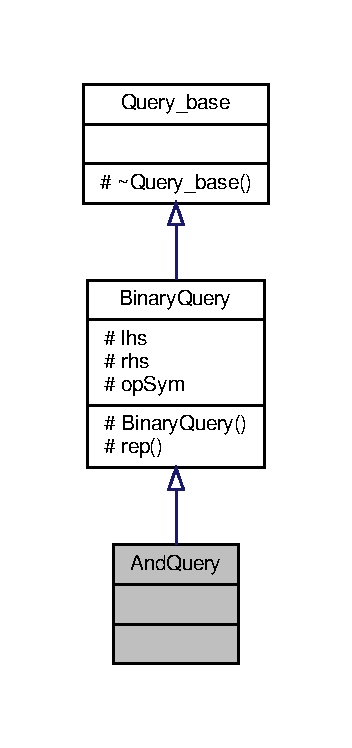
\includegraphics[width=169pt]{classAndQuery__inherit__graph}
\end{center}
\end{figure}


And\+Query 的协作图\+:\nopagebreak
\begin{figure}[H]
\begin{center}
\leavevmode
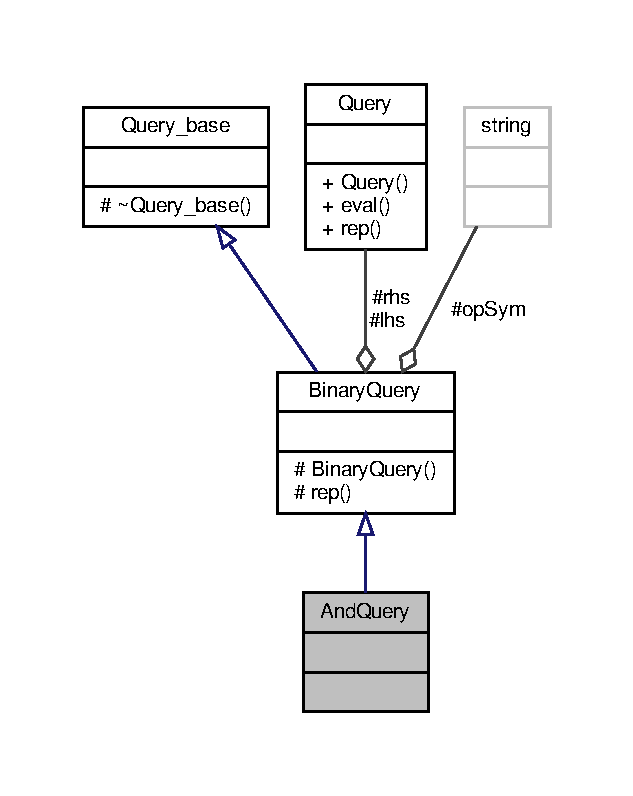
\includegraphics[width=304pt]{classAndQuery__coll__graph}
\end{center}
\end{figure}
\subsection*{友元}
\begin{DoxyCompactItemize}
\item 
\hyperlink{classQuery}{Query} \hyperlink{classAndQuery_a9669c004503314734a5671692f392812}{operator \&} (const \hyperlink{classQuery}{Query} \&, const \hyperlink{classQuery}{Query} \&)
\end{DoxyCompactItemize}
\subsection*{额外继承的成员函数}


\subsection{友元及相关函数文档}
\mbox{\Hypertarget{classAndQuery_a9669c004503314734a5671692f392812}\label{classAndQuery_a9669c004503314734a5671692f392812}} 
\index{And\+Query@{And\+Query}!operator \&@{operator \&}}
\index{operator \&@{operator \&}!And\+Query@{And\+Query}}
\subsubsection{\texorpdfstring{operator \&}{operator \&}}
{\footnotesize\ttfamily \hyperlink{classQuery}{Query} operator\& (\begin{DoxyParamCaption}\item[{const \hyperlink{classQuery}{Query} \&}]{lhs,  }\item[{const \hyperlink{classQuery}{Query} \&}]{rhs }\end{DoxyParamCaption})\hspace{0.3cm}{\ttfamily [friend]}}



该类的文档由以下文件生成\+:\begin{DoxyCompactItemize}
\item 
\hyperlink{Query_8h}{Query.\+h}\item 
\hyperlink{Query_8cpp}{Query.\+cpp}\end{DoxyCompactItemize}

\hypertarget{classBinaryQuery}{}\section{Binary\+Query类 参考}
\label{classBinaryQuery}\index{Binary\+Query@{Binary\+Query}}


{\ttfamily \#include $<$Query.\+h$>$}



类 Binary\+Query 继承关系图\+:\nopagebreak
\begin{figure}[H]
\begin{center}
\leavevmode
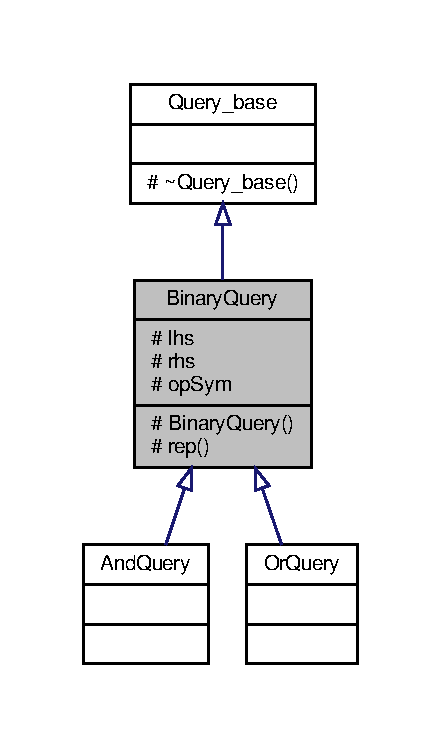
\includegraphics[width=212pt]{classBinaryQuery__inherit__graph}
\end{center}
\end{figure}


Binary\+Query 的协作图\+:\nopagebreak
\begin{figure}[H]
\begin{center}
\leavevmode
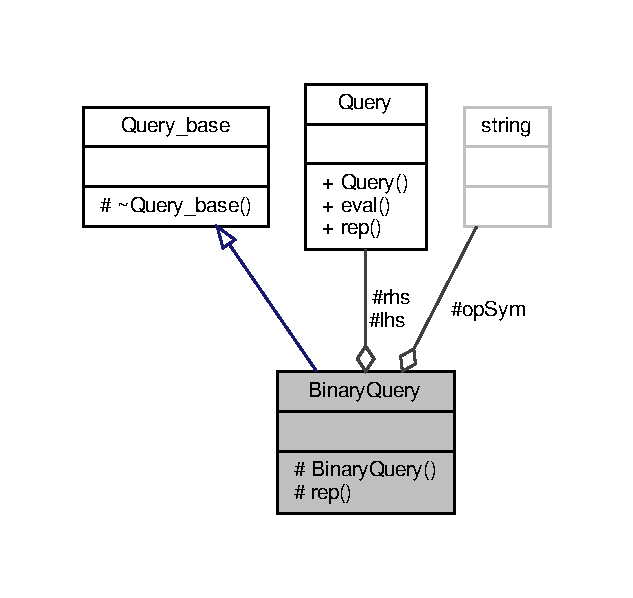
\includegraphics[width=304pt]{classBinaryQuery__coll__graph}
\end{center}
\end{figure}
\subsection*{Protected 成员函数}
\begin{DoxyCompactItemize}
\item 
\hyperlink{classBinaryQuery_aaa682971fc9991f977baf718f7697979}{Binary\+Query} (const \hyperlink{classQuery}{Query} \&l, const \hyperlink{classQuery}{Query} \&r, std\+::string s)
\item 
std\+::string \hyperlink{classBinaryQuery_ad464dd807f5b48025a48355f73b34fcd}{rep} () const
\end{DoxyCompactItemize}
\subsection*{Protected 属性}
\begin{DoxyCompactItemize}
\item 
\hyperlink{classQuery}{Query} \hyperlink{classBinaryQuery_ae1d69c3225f9ac3e16c6bb3dd59b0f07}{lhs}
\item 
\hyperlink{classQuery}{Query} \hyperlink{classBinaryQuery_a22e8a3a081421a2ea2106aa5b0541773}{rhs}
\item 
std\+::string \hyperlink{classBinaryQuery_a773bb87bb747ca84ef24af6827196271}{op\+Sym}
\end{DoxyCompactItemize}
\subsection*{额外继承的成员函数}


\subsection{构造及析构函数说明}
\mbox{\Hypertarget{classBinaryQuery_aaa682971fc9991f977baf718f7697979}\label{classBinaryQuery_aaa682971fc9991f977baf718f7697979}} 
\index{Binary\+Query@{Binary\+Query}!Binary\+Query@{Binary\+Query}}
\index{Binary\+Query@{Binary\+Query}!Binary\+Query@{Binary\+Query}}
\subsubsection{\texorpdfstring{Binary\+Query()}{BinaryQuery()}}
{\footnotesize\ttfamily Binary\+Query\+::\+Binary\+Query (\begin{DoxyParamCaption}\item[{const \hyperlink{classQuery}{Query} \&}]{l,  }\item[{const \hyperlink{classQuery}{Query} \&}]{r,  }\item[{std\+::string}]{s }\end{DoxyParamCaption})\hspace{0.3cm}{\ttfamily [inline]}, {\ttfamily [protected]}}



\subsection{成员函数说明}
\mbox{\Hypertarget{classBinaryQuery_ad464dd807f5b48025a48355f73b34fcd}\label{classBinaryQuery_ad464dd807f5b48025a48355f73b34fcd}} 
\index{Binary\+Query@{Binary\+Query}!rep@{rep}}
\index{rep@{rep}!Binary\+Query@{Binary\+Query}}
\subsubsection{\texorpdfstring{rep()}{rep()}}
{\footnotesize\ttfamily std\+::string Binary\+Query\+::rep (\begin{DoxyParamCaption}{ }\end{DoxyParamCaption}) const\hspace{0.3cm}{\ttfamily [inline]}, {\ttfamily [protected]}, {\ttfamily [virtual]}}



实现了 \hyperlink{classQuery__base}{Query\+\_\+base}.



\subsection{类成员变量说明}
\mbox{\Hypertarget{classBinaryQuery_ae1d69c3225f9ac3e16c6bb3dd59b0f07}\label{classBinaryQuery_ae1d69c3225f9ac3e16c6bb3dd59b0f07}} 
\index{Binary\+Query@{Binary\+Query}!lhs@{lhs}}
\index{lhs@{lhs}!Binary\+Query@{Binary\+Query}}
\subsubsection{\texorpdfstring{lhs}{lhs}}
{\footnotesize\ttfamily \hyperlink{classQuery}{Query} Binary\+Query\+::lhs\hspace{0.3cm}{\ttfamily [protected]}}

\mbox{\Hypertarget{classBinaryQuery_a773bb87bb747ca84ef24af6827196271}\label{classBinaryQuery_a773bb87bb747ca84ef24af6827196271}} 
\index{Binary\+Query@{Binary\+Query}!op\+Sym@{op\+Sym}}
\index{op\+Sym@{op\+Sym}!Binary\+Query@{Binary\+Query}}
\subsubsection{\texorpdfstring{op\+Sym}{opSym}}
{\footnotesize\ttfamily std\+::string Binary\+Query\+::op\+Sym\hspace{0.3cm}{\ttfamily [protected]}}

\mbox{\Hypertarget{classBinaryQuery_a22e8a3a081421a2ea2106aa5b0541773}\label{classBinaryQuery_a22e8a3a081421a2ea2106aa5b0541773}} 
\index{Binary\+Query@{Binary\+Query}!rhs@{rhs}}
\index{rhs@{rhs}!Binary\+Query@{Binary\+Query}}
\subsubsection{\texorpdfstring{rhs}{rhs}}
{\footnotesize\ttfamily \hyperlink{classQuery}{Query} Binary\+Query\+::rhs\hspace{0.3cm}{\ttfamily [protected]}}



该类的文档由以下文件生成\+:\begin{DoxyCompactItemize}
\item 
\hyperlink{Query_8h}{Query.\+h}\end{DoxyCompactItemize}

\hypertarget{classNotQuery}{}\section{Not\+Query类 参考}
\label{classNotQuery}\index{Not\+Query@{Not\+Query}}


{\ttfamily \#include $<$Query.\+h$>$}



类 Not\+Query 继承关系图\+:\nopagebreak
\begin{figure}[H]
\begin{center}
\leavevmode
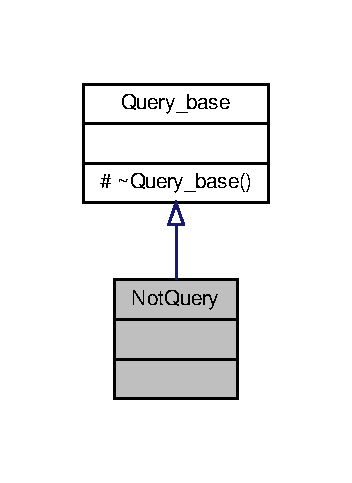
\includegraphics[width=169pt]{classNotQuery__inherit__graph}
\end{center}
\end{figure}


Not\+Query 的协作图\+:\nopagebreak
\begin{figure}[H]
\begin{center}
\leavevmode
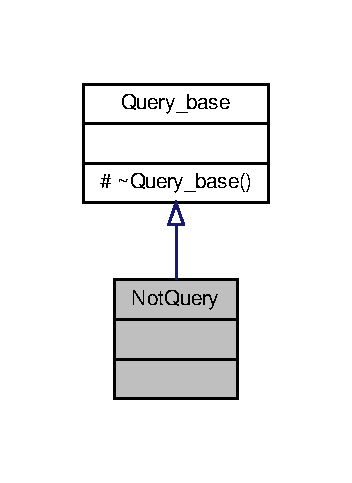
\includegraphics[width=169pt]{classNotQuery__coll__graph}
\end{center}
\end{figure}
\subsection*{友元}
\begin{DoxyCompactItemize}
\item 
\hyperlink{classQuery}{Query} \hyperlink{classNotQuery_afa815c3d9f1296e687770014302bac9a}{operator$\sim$} (const \hyperlink{classQuery}{Query} \&)
\end{DoxyCompactItemize}
\subsection*{额外继承的成员函数}


\subsection{友元及相关函数文档}
\mbox{\Hypertarget{classNotQuery_afa815c3d9f1296e687770014302bac9a}\label{classNotQuery_afa815c3d9f1296e687770014302bac9a}} 
\index{Not\+Query@{Not\+Query}!operator$\sim$@{operator$\sim$}}
\index{operator$\sim$@{operator$\sim$}!Not\+Query@{Not\+Query}}
\subsubsection{\texorpdfstring{operator$\sim$}{operator~}}
{\footnotesize\ttfamily \hyperlink{classQuery}{Query} operator$\sim$ (\begin{DoxyParamCaption}\item[{const \hyperlink{classQuery}{Query} \&}]{operand }\end{DoxyParamCaption})\hspace{0.3cm}{\ttfamily [friend]}}



该类的文档由以下文件生成\+:\begin{DoxyCompactItemize}
\item 
\hyperlink{Query_8h}{Query.\+h}\item 
\hyperlink{Query_8cpp}{Query.\+cpp}\end{DoxyCompactItemize}

\hypertarget{classOrQuery}{}\section{Or\+Query类 参考}
\label{classOrQuery}\index{Or\+Query@{Or\+Query}}


{\ttfamily \#include $<$Query.\+h$>$}



类 Or\+Query 继承关系图\+:\nopagebreak
\begin{figure}[H]
\begin{center}
\leavevmode
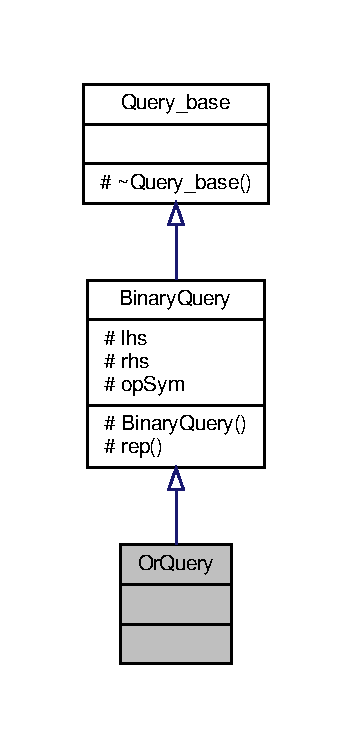
\includegraphics[width=169pt]{classOrQuery__inherit__graph}
\end{center}
\end{figure}


Or\+Query 的协作图\+:\nopagebreak
\begin{figure}[H]
\begin{center}
\leavevmode
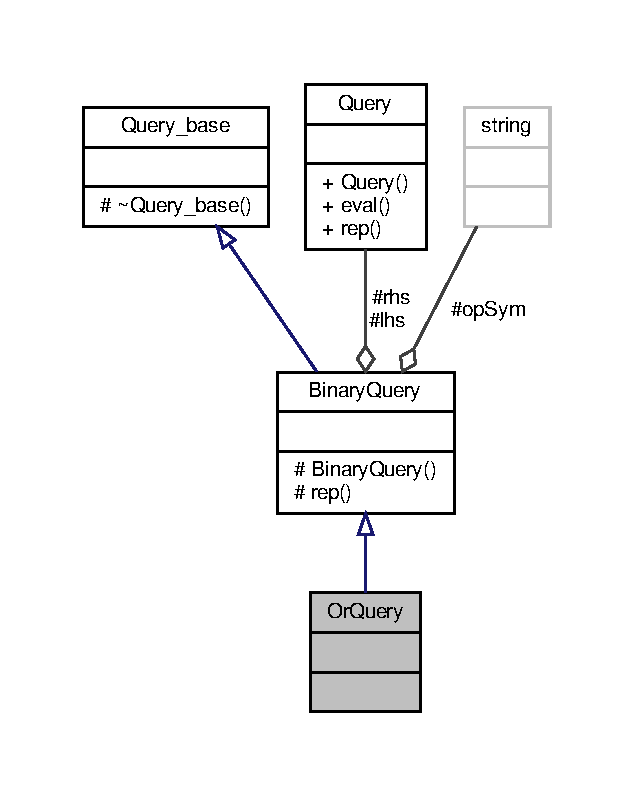
\includegraphics[width=304pt]{classOrQuery__coll__graph}
\end{center}
\end{figure}
\subsection*{友元}
\begin{DoxyCompactItemize}
\item 
\hyperlink{classQuery}{Query} \hyperlink{classOrQuery_a51852e29f84c14afd70921a21cab6074}{operator$\vert$} (const \hyperlink{classQuery}{Query} \&, const \hyperlink{classQuery}{Query} \&)
\end{DoxyCompactItemize}
\subsection*{额外继承的成员函数}


\subsection{友元及相关函数文档}
\mbox{\Hypertarget{classOrQuery_a51852e29f84c14afd70921a21cab6074}\label{classOrQuery_a51852e29f84c14afd70921a21cab6074}} 
\index{Or\+Query@{Or\+Query}!operator\texttt{"|}@{operator\texttt{"|}}}
\index{operator\texttt{"|}@{operator\texttt{"|}}!Or\+Query@{Or\+Query}}
\subsubsection{\texorpdfstring{operator\texttt{"|}}{operator|}}
{\footnotesize\ttfamily \hyperlink{classQuery}{Query} operator$\vert$ (\begin{DoxyParamCaption}\item[{const \hyperlink{classQuery}{Query} \&}]{lhs,  }\item[{const \hyperlink{classQuery}{Query} \&}]{rhs }\end{DoxyParamCaption})\hspace{0.3cm}{\ttfamily [friend]}}



该类的文档由以下文件生成\+:\begin{DoxyCompactItemize}
\item 
\hyperlink{Query_8h}{Query.\+h}\item 
\hyperlink{Query_8cpp}{Query.\+cpp}\end{DoxyCompactItemize}

\hypertarget{classQuery}{}\section{Query类 参考}
\label{classQuery}\index{Query@{Query}}


{\ttfamily \#include $<$Query.\+h$>$}



Query 的协作图\+:\nopagebreak
\begin{figure}[H]
\begin{center}
\leavevmode
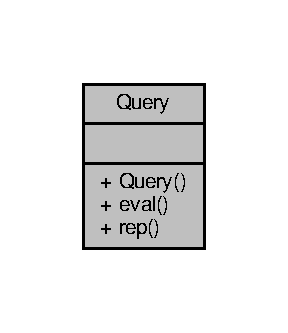
\includegraphics[width=138pt]{classQuery__coll__graph}
\end{center}
\end{figure}
\subsection*{Public 成员函数}
\begin{DoxyCompactItemize}
\item 
\hyperlink{classQuery_a60d539aa013ee1f13ff99034a1836d89}{Query} (const std\+::string \&)
\item 
\hyperlink{classQueryResult}{Query\+Result} \hyperlink{classQuery_aac65ca23ad50e878e89e831ca3c8b833}{eval} (const \hyperlink{classTextQuery}{Text\+Query} \&t) const
\item 
std\+::string \hyperlink{classQuery_a44d3f3eb47e3c7744356f12b04a6f4ac}{rep} () const
\end{DoxyCompactItemize}
\subsection*{友元}
\begin{DoxyCompactItemize}
\item 
\hyperlink{classQuery}{Query} \hyperlink{classQuery_afa815c3d9f1296e687770014302bac9a}{operator$\sim$} (const \hyperlink{classQuery}{Query} \&)
\item 
\hyperlink{classQuery}{Query} \hyperlink{classQuery_a51852e29f84c14afd70921a21cab6074}{operator$\vert$} (const \hyperlink{classQuery}{Query} \&, const \hyperlink{classQuery}{Query} \&)
\item 
\hyperlink{classQuery}{Query} \hyperlink{classQuery_a9669c004503314734a5671692f392812}{operator \&} (const \hyperlink{classQuery}{Query} \&, const \hyperlink{classQuery}{Query} \&)
\end{DoxyCompactItemize}


\subsection{构造及析构函数说明}
\mbox{\Hypertarget{classQuery_a60d539aa013ee1f13ff99034a1836d89}\label{classQuery_a60d539aa013ee1f13ff99034a1836d89}} 
\index{Query@{Query}!Query@{Query}}
\index{Query@{Query}!Query@{Query}}
\subsubsection{\texorpdfstring{Query()}{Query()}}
{\footnotesize\ttfamily Query\+::\+Query (\begin{DoxyParamCaption}\item[{const std\+::string \&}]{s }\end{DoxyParamCaption})\hspace{0.3cm}{\ttfamily [inline]}}



\subsection{成员函数说明}
\mbox{\Hypertarget{classQuery_aac65ca23ad50e878e89e831ca3c8b833}\label{classQuery_aac65ca23ad50e878e89e831ca3c8b833}} 
\index{Query@{Query}!eval@{eval}}
\index{eval@{eval}!Query@{Query}}
\subsubsection{\texorpdfstring{eval()}{eval()}}
{\footnotesize\ttfamily \hyperlink{classQueryResult}{Query\+Result} Query\+::eval (\begin{DoxyParamCaption}\item[{const \hyperlink{classTextQuery}{Text\+Query} \&}]{t }\end{DoxyParamCaption}) const\hspace{0.3cm}{\ttfamily [inline]}}

\mbox{\Hypertarget{classQuery_a44d3f3eb47e3c7744356f12b04a6f4ac}\label{classQuery_a44d3f3eb47e3c7744356f12b04a6f4ac}} 
\index{Query@{Query}!rep@{rep}}
\index{rep@{rep}!Query@{Query}}
\subsubsection{\texorpdfstring{rep()}{rep()}}
{\footnotesize\ttfamily std\+::string Query\+::rep (\begin{DoxyParamCaption}{ }\end{DoxyParamCaption}) const\hspace{0.3cm}{\ttfamily [inline]}}



\subsection{友元及相关函数文档}
\mbox{\Hypertarget{classQuery_a9669c004503314734a5671692f392812}\label{classQuery_a9669c004503314734a5671692f392812}} 
\index{Query@{Query}!operator \&@{operator \&}}
\index{operator \&@{operator \&}!Query@{Query}}
\subsubsection{\texorpdfstring{operator \&}{operator \&}}
{\footnotesize\ttfamily \hyperlink{classQuery}{Query} operator\& (\begin{DoxyParamCaption}\item[{const \hyperlink{classQuery}{Query} \&}]{lhs,  }\item[{const \hyperlink{classQuery}{Query} \&}]{rhs }\end{DoxyParamCaption})\hspace{0.3cm}{\ttfamily [friend]}}

\mbox{\Hypertarget{classQuery_a51852e29f84c14afd70921a21cab6074}\label{classQuery_a51852e29f84c14afd70921a21cab6074}} 
\index{Query@{Query}!operator\texttt{"|}@{operator\texttt{"|}}}
\index{operator\texttt{"|}@{operator\texttt{"|}}!Query@{Query}}
\subsubsection{\texorpdfstring{operator\texttt{"|}}{operator|}}
{\footnotesize\ttfamily \hyperlink{classQuery}{Query} operator$\vert$ (\begin{DoxyParamCaption}\item[{const \hyperlink{classQuery}{Query} \&}]{lhs,  }\item[{const \hyperlink{classQuery}{Query} \&}]{rhs }\end{DoxyParamCaption})\hspace{0.3cm}{\ttfamily [friend]}}

\mbox{\Hypertarget{classQuery_afa815c3d9f1296e687770014302bac9a}\label{classQuery_afa815c3d9f1296e687770014302bac9a}} 
\index{Query@{Query}!operator$\sim$@{operator$\sim$}}
\index{operator$\sim$@{operator$\sim$}!Query@{Query}}
\subsubsection{\texorpdfstring{operator$\sim$}{operator~}}
{\footnotesize\ttfamily \hyperlink{classQuery}{Query} operator$\sim$ (\begin{DoxyParamCaption}\item[{const \hyperlink{classQuery}{Query} \&}]{operand }\end{DoxyParamCaption})\hspace{0.3cm}{\ttfamily [friend]}}



该类的文档由以下文件生成\+:\begin{DoxyCompactItemize}
\item 
\hyperlink{Query_8h}{Query.\+h}\end{DoxyCompactItemize}

\hypertarget{classQuery__base}{}\section{Query\+\_\+base类 参考}
\label{classQuery__base}\index{Query\+\_\+base@{Query\+\_\+base}}


{\ttfamily \#include $<$Query.\+h$>$}



类 Query\+\_\+base 继承关系图\+:\nopagebreak
\begin{figure}[H]
\begin{center}
\leavevmode
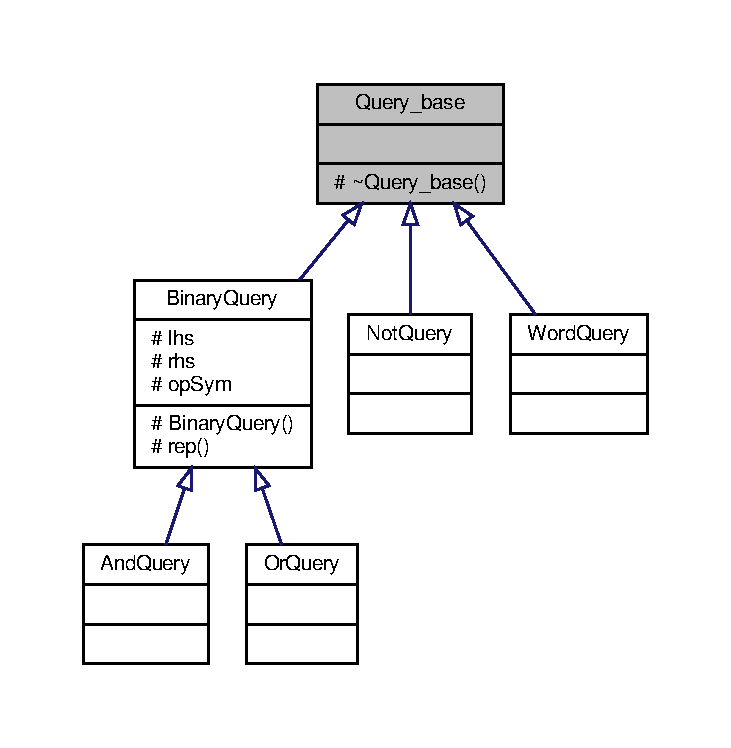
\includegraphics[width=350pt]{classQuery__base__inherit__graph}
\end{center}
\end{figure}


Query\+\_\+base 的协作图\+:\nopagebreak
\begin{figure}[H]
\begin{center}
\leavevmode
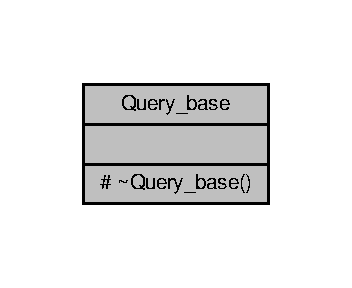
\includegraphics[width=169pt]{classQuery__base__coll__graph}
\end{center}
\end{figure}
\subsection*{Protected 类型}
\begin{DoxyCompactItemize}
\item 
typedef \hyperlink{classTextQuery_a504c1be8d67d4fcf4c205999e2377262}{Text\+Query\+::line\+\_\+no} \hyperlink{classQuery__base_a653b9dc8622a918b227c9f30dc636fba}{line\+\_\+no}
\end{DoxyCompactItemize}
\subsection*{Protected 成员函数}
\begin{DoxyCompactItemize}
\item 
virtual \hyperlink{classQuery__base_aa935ca8c8ea768ea3c5bd8d1df6f0c27}{$\sim$\+Query\+\_\+base} ()
\end{DoxyCompactItemize}
\subsection*{友元}
\begin{DoxyCompactItemize}
\item 
class \hyperlink{classQuery__base_a0de80064a367adf51ab09f7a9b6de05a}{Query}
\end{DoxyCompactItemize}


\subsection{成员类型定义说明}
\mbox{\Hypertarget{classQuery__base_a653b9dc8622a918b227c9f30dc636fba}\label{classQuery__base_a653b9dc8622a918b227c9f30dc636fba}} 
\index{Query\+\_\+base@{Query\+\_\+base}!line\+\_\+no@{line\+\_\+no}}
\index{line\+\_\+no@{line\+\_\+no}!Query\+\_\+base@{Query\+\_\+base}}
\subsubsection{\texorpdfstring{line\+\_\+no}{line\_no}}
{\footnotesize\ttfamily typedef \hyperlink{classTextQuery_a504c1be8d67d4fcf4c205999e2377262}{Text\+Query\+::line\+\_\+no} \hyperlink{classQuery__base_a653b9dc8622a918b227c9f30dc636fba}{Query\+\_\+base\+::line\+\_\+no}\hspace{0.3cm}{\ttfamily [protected]}}



\subsection{构造及析构函数说明}
\mbox{\Hypertarget{classQuery__base_aa935ca8c8ea768ea3c5bd8d1df6f0c27}\label{classQuery__base_aa935ca8c8ea768ea3c5bd8d1df6f0c27}} 
\index{Query\+\_\+base@{Query\+\_\+base}!````~Query\+\_\+base@{$\sim$\+Query\+\_\+base}}
\index{````~Query\+\_\+base@{$\sim$\+Query\+\_\+base}!Query\+\_\+base@{Query\+\_\+base}}
\subsubsection{\texorpdfstring{$\sim$\+Query\+\_\+base()}{~Query\_base()}}
{\footnotesize\ttfamily virtual Query\+\_\+base\+::$\sim$\+Query\+\_\+base (\begin{DoxyParamCaption}{ }\end{DoxyParamCaption})\hspace{0.3cm}{\ttfamily [inline]}, {\ttfamily [protected]}, {\ttfamily [virtual]}}



\subsection{友元及相关函数文档}
\mbox{\Hypertarget{classQuery__base_a0de80064a367adf51ab09f7a9b6de05a}\label{classQuery__base_a0de80064a367adf51ab09f7a9b6de05a}} 
\index{Query\+\_\+base@{Query\+\_\+base}!Query@{Query}}
\index{Query@{Query}!Query\+\_\+base@{Query\+\_\+base}}
\subsubsection{\texorpdfstring{Query}{Query}}
{\footnotesize\ttfamily friend class \hyperlink{classQuery}{Query}\hspace{0.3cm}{\ttfamily [friend]}}



该类的文档由以下文件生成\+:\begin{DoxyCompactItemize}
\item 
\hyperlink{Query_8h}{Query.\+h}\end{DoxyCompactItemize}

\hypertarget{classQueryResult}{}\section{Query\+Result类 参考}
\label{classQueryResult}\index{Query\+Result@{Query\+Result}}


{\ttfamily \#include $<$Query\+Result.\+h$>$}



Query\+Result 的协作图\+:\nopagebreak
\begin{figure}[H]
\begin{center}
\leavevmode
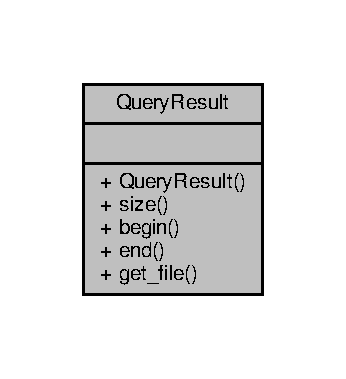
\includegraphics[width=166pt]{classQueryResult__coll__graph}
\end{center}
\end{figure}
\subsection*{Public 类型}
\begin{DoxyCompactItemize}
\item 
typedef std\+::vector$<$ std\+::string $>$\+::size\+\_\+type \hyperlink{classQueryResult_a34e6c64fb173f43499443469009c262f}{line\+\_\+no}
\item 
typedef std\+::set$<$ \hyperlink{classQueryResult_a34e6c64fb173f43499443469009c262f}{line\+\_\+no} $>$\+::const\+\_\+iterator \hyperlink{classQueryResult_a863424dfa74a1048fdcb636a98aea670}{line\+\_\+it}
\end{DoxyCompactItemize}
\subsection*{Public 成员函数}
\begin{DoxyCompactItemize}
\item 
\hyperlink{classQueryResult_a9712669ad32f23c0875c1a2b4dc55ef2}{Query\+Result} (std\+::string s, std\+::shared\+\_\+ptr$<$ std\+::set$<$ \hyperlink{classQueryResult_a34e6c64fb173f43499443469009c262f}{line\+\_\+no} $>$ $>$ p, std\+::shared\+\_\+ptr$<$ std\+::vector$<$ std\+::string $>$ $>$ f)
\item 
std\+::set$<$ \hyperlink{classQueryResult_a34e6c64fb173f43499443469009c262f}{line\+\_\+no} $>$\+::size\+\_\+type \hyperlink{classQueryResult_af4d3e42b7cf43c88783069d484796052}{size} () const
\item 
\hyperlink{classQueryResult_a863424dfa74a1048fdcb636a98aea670}{line\+\_\+it} \hyperlink{classQueryResult_ac78944666adea9b2443e66bea6546857}{begin} () const
\item 
\hyperlink{classQueryResult_a863424dfa74a1048fdcb636a98aea670}{line\+\_\+it} \hyperlink{classQueryResult_a5ba21e424a2db6b4e91bc0079b165b70}{end} () const
\item 
std\+::shared\+\_\+ptr$<$ std\+::vector$<$ std\+::string $>$ $>$ \hyperlink{classQueryResult_af9b8d280bfe034dd1f7046036a98df93}{get\+\_\+file} ()
\end{DoxyCompactItemize}
\subsection*{友元}
\begin{DoxyCompactItemize}
\item 
std\+::ostream \& \hyperlink{classQueryResult_ab20f9885050aa16c68eaeff6f8d9db7d}{print} (std\+::ostream \&, const \hyperlink{classQueryResult}{Query\+Result} \&)
\end{DoxyCompactItemize}


\subsection{成员类型定义说明}
\mbox{\Hypertarget{classQueryResult_a863424dfa74a1048fdcb636a98aea670}\label{classQueryResult_a863424dfa74a1048fdcb636a98aea670}} 
\index{Query\+Result@{Query\+Result}!line\+\_\+it@{line\+\_\+it}}
\index{line\+\_\+it@{line\+\_\+it}!Query\+Result@{Query\+Result}}
\subsubsection{\texorpdfstring{line\+\_\+it}{line\_it}}
{\footnotesize\ttfamily typedef std\+::set$<$\hyperlink{classQueryResult_a34e6c64fb173f43499443469009c262f}{line\+\_\+no}$>$\+::const\+\_\+iterator \hyperlink{classQueryResult_a863424dfa74a1048fdcb636a98aea670}{Query\+Result\+::line\+\_\+it}}

\mbox{\Hypertarget{classQueryResult_a34e6c64fb173f43499443469009c262f}\label{classQueryResult_a34e6c64fb173f43499443469009c262f}} 
\index{Query\+Result@{Query\+Result}!line\+\_\+no@{line\+\_\+no}}
\index{line\+\_\+no@{line\+\_\+no}!Query\+Result@{Query\+Result}}
\subsubsection{\texorpdfstring{line\+\_\+no}{line\_no}}
{\footnotesize\ttfamily typedef std\+::vector$<$std\+::string$>$\+::size\+\_\+type \hyperlink{classQueryResult_a34e6c64fb173f43499443469009c262f}{Query\+Result\+::line\+\_\+no}}



\subsection{构造及析构函数说明}
\mbox{\Hypertarget{classQueryResult_a9712669ad32f23c0875c1a2b4dc55ef2}\label{classQueryResult_a9712669ad32f23c0875c1a2b4dc55ef2}} 
\index{Query\+Result@{Query\+Result}!Query\+Result@{Query\+Result}}
\index{Query\+Result@{Query\+Result}!Query\+Result@{Query\+Result}}
\subsubsection{\texorpdfstring{Query\+Result()}{QueryResult()}}
{\footnotesize\ttfamily Query\+Result\+::\+Query\+Result (\begin{DoxyParamCaption}\item[{std\+::string}]{s,  }\item[{std\+::shared\+\_\+ptr$<$ std\+::set$<$ \hyperlink{classQueryResult_a34e6c64fb173f43499443469009c262f}{line\+\_\+no} $>$ $>$}]{p,  }\item[{std\+::shared\+\_\+ptr$<$ std\+::vector$<$ std\+::string $>$ $>$}]{f }\end{DoxyParamCaption})\hspace{0.3cm}{\ttfamily [inline]}}



\subsection{成员函数说明}
\mbox{\Hypertarget{classQueryResult_ac78944666adea9b2443e66bea6546857}\label{classQueryResult_ac78944666adea9b2443e66bea6546857}} 
\index{Query\+Result@{Query\+Result}!begin@{begin}}
\index{begin@{begin}!Query\+Result@{Query\+Result}}
\subsubsection{\texorpdfstring{begin()}{begin()}}
{\footnotesize\ttfamily \hyperlink{classQueryResult_a863424dfa74a1048fdcb636a98aea670}{line\+\_\+it} Query\+Result\+::begin (\begin{DoxyParamCaption}{ }\end{DoxyParamCaption}) const\hspace{0.3cm}{\ttfamily [inline]}}

\mbox{\Hypertarget{classQueryResult_a5ba21e424a2db6b4e91bc0079b165b70}\label{classQueryResult_a5ba21e424a2db6b4e91bc0079b165b70}} 
\index{Query\+Result@{Query\+Result}!end@{end}}
\index{end@{end}!Query\+Result@{Query\+Result}}
\subsubsection{\texorpdfstring{end()}{end()}}
{\footnotesize\ttfamily \hyperlink{classQueryResult_a863424dfa74a1048fdcb636a98aea670}{line\+\_\+it} Query\+Result\+::end (\begin{DoxyParamCaption}{ }\end{DoxyParamCaption}) const\hspace{0.3cm}{\ttfamily [inline]}}

\mbox{\Hypertarget{classQueryResult_af9b8d280bfe034dd1f7046036a98df93}\label{classQueryResult_af9b8d280bfe034dd1f7046036a98df93}} 
\index{Query\+Result@{Query\+Result}!get\+\_\+file@{get\+\_\+file}}
\index{get\+\_\+file@{get\+\_\+file}!Query\+Result@{Query\+Result}}
\subsubsection{\texorpdfstring{get\+\_\+file()}{get\_file()}}
{\footnotesize\ttfamily std\+::shared\+\_\+ptr$<$std\+::vector$<$std\+::string$>$ $>$ Query\+Result\+::get\+\_\+file (\begin{DoxyParamCaption}{ }\end{DoxyParamCaption})\hspace{0.3cm}{\ttfamily [inline]}}

\mbox{\Hypertarget{classQueryResult_af4d3e42b7cf43c88783069d484796052}\label{classQueryResult_af4d3e42b7cf43c88783069d484796052}} 
\index{Query\+Result@{Query\+Result}!size@{size}}
\index{size@{size}!Query\+Result@{Query\+Result}}
\subsubsection{\texorpdfstring{size()}{size()}}
{\footnotesize\ttfamily std\+::set$<$\hyperlink{classQueryResult_a34e6c64fb173f43499443469009c262f}{line\+\_\+no}$>$\+::size\+\_\+type Query\+Result\+::size (\begin{DoxyParamCaption}{ }\end{DoxyParamCaption}) const\hspace{0.3cm}{\ttfamily [inline]}}



\subsection{友元及相关函数文档}
\mbox{\Hypertarget{classQueryResult_ab20f9885050aa16c68eaeff6f8d9db7d}\label{classQueryResult_ab20f9885050aa16c68eaeff6f8d9db7d}} 
\index{Query\+Result@{Query\+Result}!print@{print}}
\index{print@{print}!Query\+Result@{Query\+Result}}
\subsubsection{\texorpdfstring{print}{print}}
{\footnotesize\ttfamily std\+::ostream\& print (\begin{DoxyParamCaption}\item[{std\+::ostream \&}]{,  }\item[{const \hyperlink{classQueryResult}{Query\+Result} \&}]{ }\end{DoxyParamCaption})\hspace{0.3cm}{\ttfamily [friend]}}



该类的文档由以下文件生成\+:\begin{DoxyCompactItemize}
\item 
\hyperlink{QueryResult_8h}{Query\+Result.\+h}\end{DoxyCompactItemize}

\hypertarget{classTextQuery}{}\section{Text\+Query类 参考}
\label{classTextQuery}\index{Text\+Query@{Text\+Query}}


{\ttfamily \#include $<$Text\+Query.\+h$>$}



Text\+Query 的协作图\+:\nopagebreak
\begin{figure}[H]
\begin{center}
\leavevmode
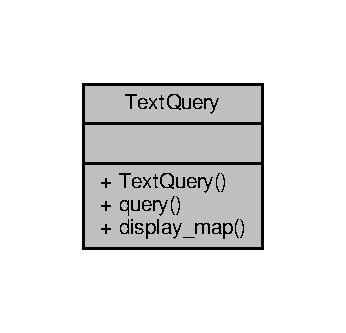
\includegraphics[width=166pt]{classTextQuery__coll__graph}
\end{center}
\end{figure}
\subsection*{Public 类型}
\begin{DoxyCompactItemize}
\item 
using \hyperlink{classTextQuery_a504c1be8d67d4fcf4c205999e2377262}{line\+\_\+no} = std\+::vector$<$ std\+::string $>$\+::size\+\_\+type
\end{DoxyCompactItemize}
\subsection*{Public 成员函数}
\begin{DoxyCompactItemize}
\item 
\hyperlink{classTextQuery_a7362fe39ff27f72b5aa4127459318606}{Text\+Query} (std\+::ifstream \&)
\item 
\hyperlink{classQueryResult}{Query\+Result} \hyperlink{classTextQuery_acdbf168c6de152095bce2ce3aaa11d1d}{query} (const std\+::string \&) const
\item 
void \hyperlink{classTextQuery_a481824aee58568ba51455e3131f479dd}{display\+\_\+map} ()
\end{DoxyCompactItemize}


\subsection{成员类型定义说明}
\mbox{\Hypertarget{classTextQuery_a504c1be8d67d4fcf4c205999e2377262}\label{classTextQuery_a504c1be8d67d4fcf4c205999e2377262}} 
\index{Text\+Query@{Text\+Query}!line\+\_\+no@{line\+\_\+no}}
\index{line\+\_\+no@{line\+\_\+no}!Text\+Query@{Text\+Query}}
\subsubsection{\texorpdfstring{line\+\_\+no}{line\_no}}
{\footnotesize\ttfamily using \hyperlink{classTextQuery_a504c1be8d67d4fcf4c205999e2377262}{Text\+Query\+::line\+\_\+no} =  std\+::vector$<$std\+::string$>$\+::size\+\_\+type}



\subsection{构造及析构函数说明}
\mbox{\Hypertarget{classTextQuery_a7362fe39ff27f72b5aa4127459318606}\label{classTextQuery_a7362fe39ff27f72b5aa4127459318606}} 
\index{Text\+Query@{Text\+Query}!Text\+Query@{Text\+Query}}
\index{Text\+Query@{Text\+Query}!Text\+Query@{Text\+Query}}
\subsubsection{\texorpdfstring{Text\+Query()}{TextQuery()}}
{\footnotesize\ttfamily Text\+Query\+::\+Text\+Query (\begin{DoxyParamCaption}\item[{std\+::ifstream \&}]{ }\end{DoxyParamCaption})}



\subsection{成员函数说明}
\mbox{\Hypertarget{classTextQuery_a481824aee58568ba51455e3131f479dd}\label{classTextQuery_a481824aee58568ba51455e3131f479dd}} 
\index{Text\+Query@{Text\+Query}!display\+\_\+map@{display\+\_\+map}}
\index{display\+\_\+map@{display\+\_\+map}!Text\+Query@{Text\+Query}}
\subsubsection{\texorpdfstring{display\+\_\+map()}{display\_map()}}
{\footnotesize\ttfamily void Text\+Query\+::display\+\_\+map (\begin{DoxyParamCaption}{ }\end{DoxyParamCaption})}

\mbox{\Hypertarget{classTextQuery_acdbf168c6de152095bce2ce3aaa11d1d}\label{classTextQuery_acdbf168c6de152095bce2ce3aaa11d1d}} 
\index{Text\+Query@{Text\+Query}!query@{query}}
\index{query@{query}!Text\+Query@{Text\+Query}}
\subsubsection{\texorpdfstring{query()}{query()}}
{\footnotesize\ttfamily \hyperlink{classQueryResult}{Query\+Result} Text\+Query\+::query (\begin{DoxyParamCaption}\item[{const std\+::string \&}]{ }\end{DoxyParamCaption}) const}



该类的文档由以下文件生成\+:\begin{DoxyCompactItemize}
\item 
\hyperlink{TextQuery_8h}{Text\+Query.\+h}\item 
\hyperlink{TextQuery_8cpp}{Text\+Query.\+cpp}\end{DoxyCompactItemize}

\hypertarget{classWordQuery}{}\section{Word\+Query类 参考}
\label{classWordQuery}\index{Word\+Query@{Word\+Query}}


{\ttfamily \#include $<$Query.\+h$>$}



类 Word\+Query 继承关系图\+:\nopagebreak
\begin{figure}[H]
\begin{center}
\leavevmode
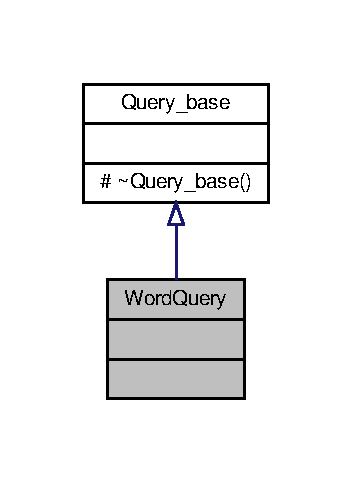
\includegraphics[width=169pt]{classWordQuery__inherit__graph}
\end{center}
\end{figure}


Word\+Query 的协作图\+:\nopagebreak
\begin{figure}[H]
\begin{center}
\leavevmode
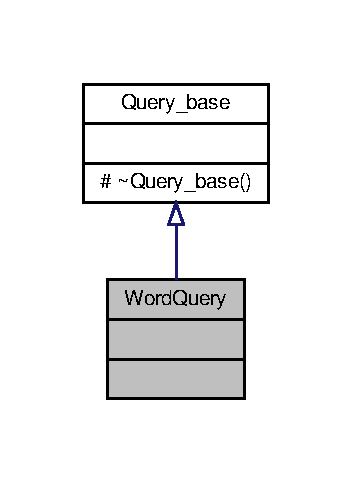
\includegraphics[width=169pt]{classWordQuery__coll__graph}
\end{center}
\end{figure}
\subsection*{友元}
\begin{DoxyCompactItemize}
\item 
class \hyperlink{classWordQuery_a0de80064a367adf51ab09f7a9b6de05a}{Query}
\end{DoxyCompactItemize}
\subsection*{额外继承的成员函数}


\subsection{友元及相关函数文档}
\mbox{\Hypertarget{classWordQuery_a0de80064a367adf51ab09f7a9b6de05a}\label{classWordQuery_a0de80064a367adf51ab09f7a9b6de05a}} 
\index{Word\+Query@{Word\+Query}!Query@{Query}}
\index{Query@{Query}!Word\+Query@{Word\+Query}}
\subsubsection{\texorpdfstring{Query}{Query}}
{\footnotesize\ttfamily friend class \hyperlink{classQuery}{Query}\hspace{0.3cm}{\ttfamily [friend]}}



该类的文档由以下文件生成\+:\begin{DoxyCompactItemize}
\item 
\hyperlink{Query_8h}{Query.\+h}\end{DoxyCompactItemize}

\chapter{文件说明}
\hypertarget{and__orQueryTest_8cpp}{}\section{and\+\_\+or\+Query\+Test.\+cpp 文件参考}
\label{and__orQueryTest_8cpp}\index{and\+\_\+or\+Query\+Test.\+cpp@{and\+\_\+or\+Query\+Test.\+cpp}}
{\ttfamily \#include \char`\"{}Query.\+h\char`\"{}}\newline
{\ttfamily \#include \char`\"{}Text\+Query.\+h\char`\"{}}\newline
{\ttfamily \#include $<$string$>$}\newline
{\ttfamily \#include $<$set$>$}\newline
{\ttfamily \#include $<$iostream$>$}\newline
and\+\_\+or\+Query\+Test.\+cpp 的引用(Include)关系图\+:\nopagebreak
\begin{figure}[H]
\begin{center}
\leavevmode
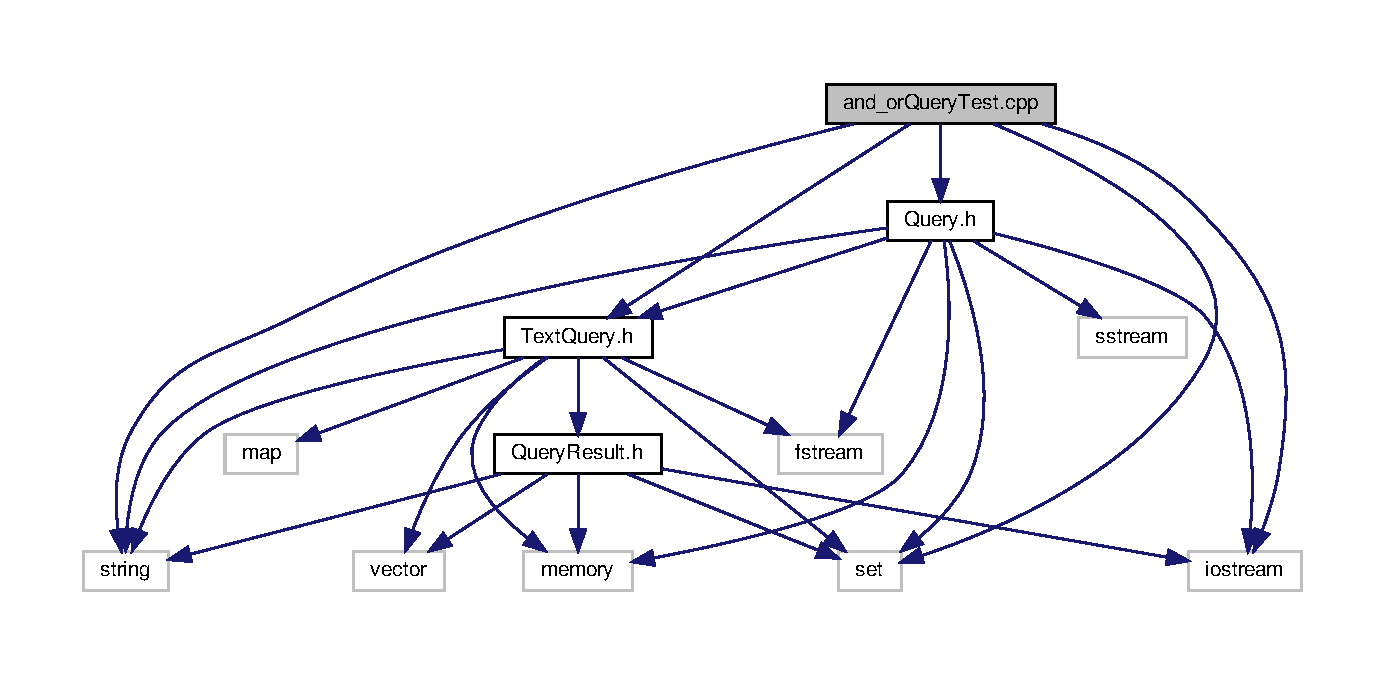
\includegraphics[width=350pt]{and__orQueryTest_8cpp__incl}
\end{center}
\end{figure}
\subsection*{函数}
\begin{DoxyCompactItemize}
\item 
int \hyperlink{and__orQueryTest_8cpp_a3c04138a5bfe5d72780bb7e82a18e627}{main} (int argc, char $\ast$$\ast$argv)
\end{DoxyCompactItemize}


\subsection{函数说明}
\mbox{\Hypertarget{and__orQueryTest_8cpp_a3c04138a5bfe5d72780bb7e82a18e627}\label{and__orQueryTest_8cpp_a3c04138a5bfe5d72780bb7e82a18e627}} 
\index{and\+\_\+or\+Query\+Test.\+cpp@{and\+\_\+or\+Query\+Test.\+cpp}!main@{main}}
\index{main@{main}!and\+\_\+or\+Query\+Test.\+cpp@{and\+\_\+or\+Query\+Test.\+cpp}}
\subsubsection{\texorpdfstring{main()}{main()}}
{\footnotesize\ttfamily int main (\begin{DoxyParamCaption}\item[{int}]{argc,  }\item[{char $\ast$$\ast$}]{argv }\end{DoxyParamCaption})}


\hypertarget{andQueryTest_8cpp}{}\section{and\+Query\+Test.\+cpp 文件参考}
\label{andQueryTest_8cpp}\index{and\+Query\+Test.\+cpp@{and\+Query\+Test.\+cpp}}
{\ttfamily \#include \char`\"{}Query.\+h\char`\"{}}\newline
{\ttfamily \#include \char`\"{}Text\+Query.\+h\char`\"{}}\newline
{\ttfamily \#include $<$string$>$}\newline
{\ttfamily \#include $<$iostream$>$}\newline
{\ttfamily \#include $<$set$>$}\newline
and\+Query\+Test.\+cpp 的引用(Include)关系图\+:\nopagebreak
\begin{figure}[H]
\begin{center}
\leavevmode
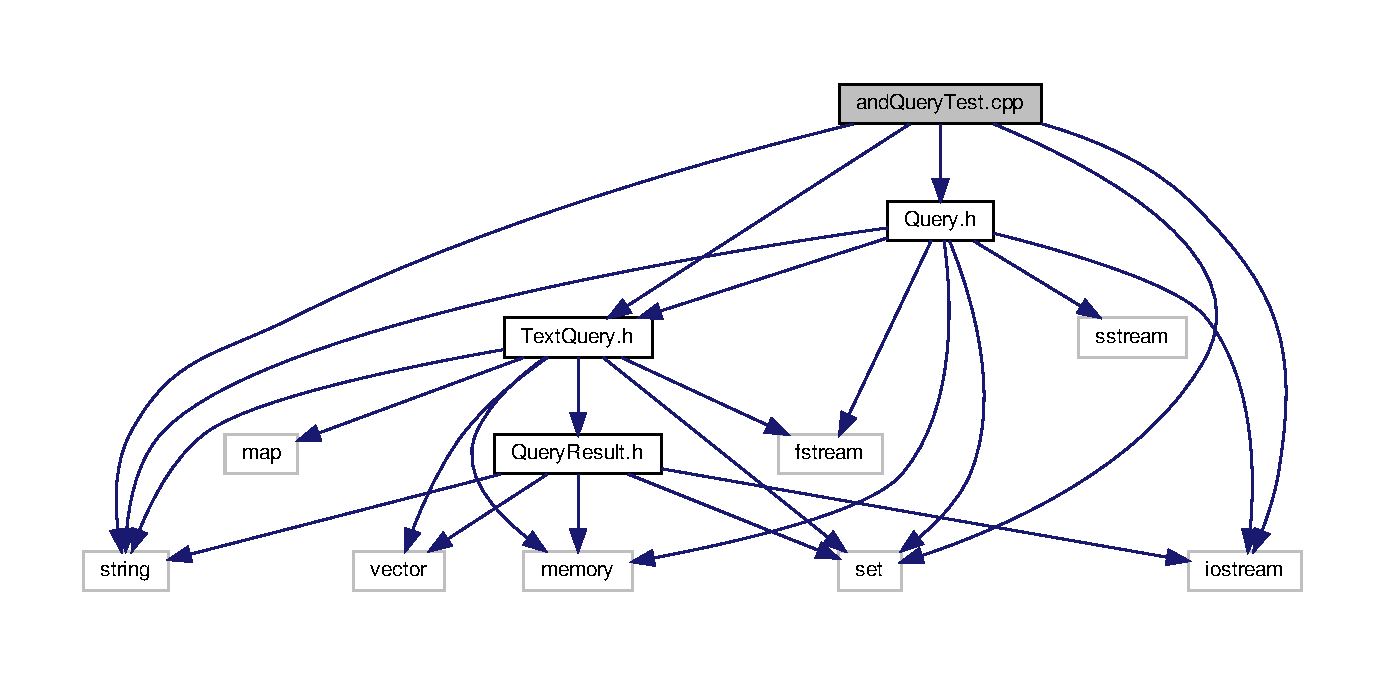
\includegraphics[width=350pt]{andQueryTest_8cpp__incl}
\end{center}
\end{figure}
\subsection*{函数}
\begin{DoxyCompactItemize}
\item 
int \hyperlink{andQueryTest_8cpp_a3c04138a5bfe5d72780bb7e82a18e627}{main} (int argc, char $\ast$$\ast$argv)
\end{DoxyCompactItemize}


\subsection{函数说明}
\mbox{\Hypertarget{andQueryTest_8cpp_a3c04138a5bfe5d72780bb7e82a18e627}\label{andQueryTest_8cpp_a3c04138a5bfe5d72780bb7e82a18e627}} 
\index{and\+Query\+Test.\+cpp@{and\+Query\+Test.\+cpp}!main@{main}}
\index{main@{main}!and\+Query\+Test.\+cpp@{and\+Query\+Test.\+cpp}}
\subsubsection{\texorpdfstring{main()}{main()}}
{\footnotesize\ttfamily int main (\begin{DoxyParamCaption}\item[{int}]{argc,  }\item[{char $\ast$$\ast$}]{argv }\end{DoxyParamCaption})}


\hypertarget{get__print_8cpp}{}\section{get\+\_\+print.\+cpp 文件参考}
\label{get__print_8cpp}\index{get\+\_\+print.\+cpp@{get\+\_\+print.\+cpp}}
{\ttfamily \#include \char`\"{}Query.\+h\char`\"{}}\newline
{\ttfamily \#include \char`\"{}Text\+Query.\+h\char`\"{}}\newline
{\ttfamily \#include $<$string$>$}\newline
{\ttfamily \#include $<$iostream$>$}\newline
{\ttfamily \#include $<$fstream$>$}\newline
{\ttfamily \#include $<$stdexcept$>$}\newline
get\+\_\+print.\+cpp 的引用(Include)关系图\+:\nopagebreak
\begin{figure}[H]
\begin{center}
\leavevmode
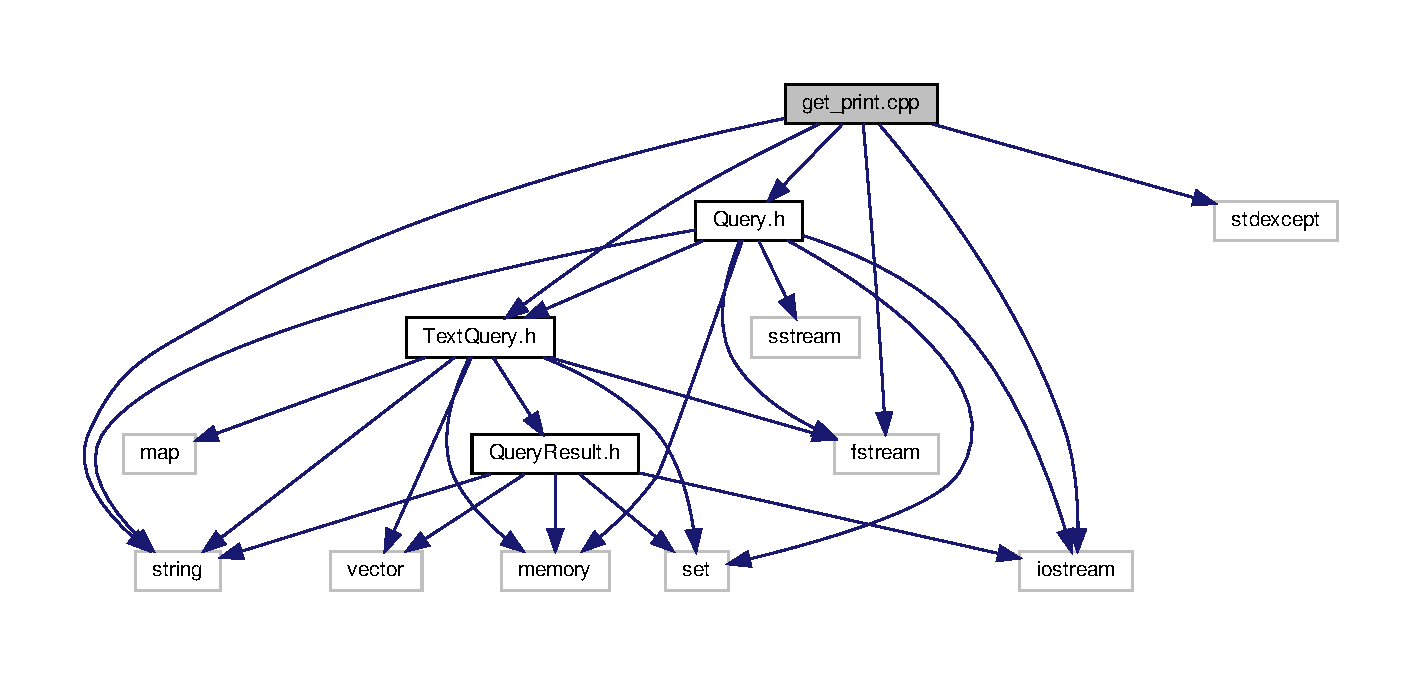
\includegraphics[width=350pt]{get__print_8cpp__incl}
\end{center}
\end{figure}
\subsection*{函数}
\begin{DoxyCompactItemize}
\item 
\hyperlink{classTextQuery}{Text\+Query} \hyperlink{get__print_8cpp_ad5978e809629ddc9e1738325e5243aee}{get\+\_\+file} (int argc, char $\ast$$\ast$argv)
\item 
bool \hyperlink{get__print_8cpp_a7a4d61ae44d51ba5d5746daa37863566}{get\+\_\+word} (string \&s1)
\item 
bool \hyperlink{get__print_8cpp_aed77932d00688b30dc55d10fa343f946}{get\+\_\+words} (string \&s1, string \&s2)
\end{DoxyCompactItemize}


\subsection{函数说明}
\mbox{\Hypertarget{get__print_8cpp_ad5978e809629ddc9e1738325e5243aee}\label{get__print_8cpp_ad5978e809629ddc9e1738325e5243aee}} 
\index{get\+\_\+print.\+cpp@{get\+\_\+print.\+cpp}!get\+\_\+file@{get\+\_\+file}}
\index{get\+\_\+file@{get\+\_\+file}!get\+\_\+print.\+cpp@{get\+\_\+print.\+cpp}}
\subsubsection{\texorpdfstring{get\+\_\+file()}{get\_file()}}
{\footnotesize\ttfamily \hyperlink{classTextQuery}{Text\+Query} get\+\_\+file (\begin{DoxyParamCaption}\item[{int}]{argc,  }\item[{char $\ast$$\ast$}]{argv }\end{DoxyParamCaption})}

\mbox{\Hypertarget{get__print_8cpp_a7a4d61ae44d51ba5d5746daa37863566}\label{get__print_8cpp_a7a4d61ae44d51ba5d5746daa37863566}} 
\index{get\+\_\+print.\+cpp@{get\+\_\+print.\+cpp}!get\+\_\+word@{get\+\_\+word}}
\index{get\+\_\+word@{get\+\_\+word}!get\+\_\+print.\+cpp@{get\+\_\+print.\+cpp}}
\subsubsection{\texorpdfstring{get\+\_\+word()}{get\_word()}}
{\footnotesize\ttfamily bool get\+\_\+word (\begin{DoxyParamCaption}\item[{string \&}]{s1 }\end{DoxyParamCaption})}

\mbox{\Hypertarget{get__print_8cpp_aed77932d00688b30dc55d10fa343f946}\label{get__print_8cpp_aed77932d00688b30dc55d10fa343f946}} 
\index{get\+\_\+print.\+cpp@{get\+\_\+print.\+cpp}!get\+\_\+words@{get\+\_\+words}}
\index{get\+\_\+words@{get\+\_\+words}!get\+\_\+print.\+cpp@{get\+\_\+print.\+cpp}}
\subsubsection{\texorpdfstring{get\+\_\+words()}{get\_words()}}
{\footnotesize\ttfamily bool get\+\_\+words (\begin{DoxyParamCaption}\item[{string \&}]{s1,  }\item[{string \&}]{s2 }\end{DoxyParamCaption})}


\hypertarget{make__plural_8h}{}\section{make\+\_\+plural.\+h 文件参考}
\label{make__plural_8h}\index{make\+\_\+plural.\+h@{make\+\_\+plural.\+h}}
{\ttfamily \#include $<$cstddef$>$}\newline
{\ttfamily \#include $<$string$>$}\newline
{\ttfamily \#include $<$iostream$>$}\newline
make\+\_\+plural.\+h 的引用(Include)关系图\+:\nopagebreak
\begin{figure}[H]
\begin{center}
\leavevmode
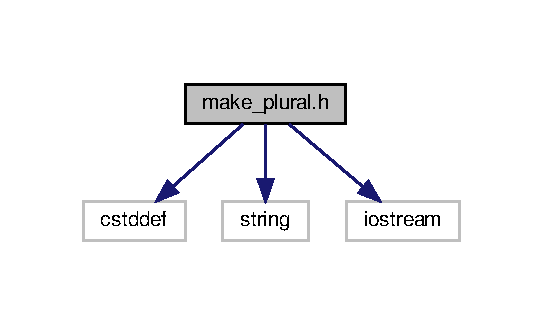
\includegraphics[width=261pt]{make__plural_8h__incl}
\end{center}
\end{figure}
此图展示该文件直接或间接的被哪些文件引用了\+:\nopagebreak
\begin{figure}[H]
\begin{center}
\leavevmode
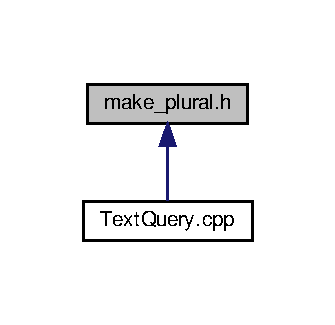
\includegraphics[width=161pt]{make__plural_8h__dep__incl}
\end{center}
\end{figure}
\subsection*{函数}
\begin{DoxyCompactItemize}
\item 
string \hyperlink{make__plural_8h_a105b78656133e09436df81a73a757a97}{make\+\_\+plural} (size\+\_\+t ctr, const string \&word, const string \&ending)
\end{DoxyCompactItemize}


\subsection{函数说明}
\mbox{\Hypertarget{make__plural_8h_a105b78656133e09436df81a73a757a97}\label{make__plural_8h_a105b78656133e09436df81a73a757a97}} 
\index{make\+\_\+plural.\+h@{make\+\_\+plural.\+h}!make\+\_\+plural@{make\+\_\+plural}}
\index{make\+\_\+plural@{make\+\_\+plural}!make\+\_\+plural.\+h@{make\+\_\+plural.\+h}}
\subsubsection{\texorpdfstring{make\+\_\+plural()}{make\_plural()}}
{\footnotesize\ttfamily string make\+\_\+plural (\begin{DoxyParamCaption}\item[{size\+\_\+t}]{ctr,  }\item[{const string \&}]{word,  }\item[{const string \&}]{ending }\end{DoxyParamCaption})\hspace{0.3cm}{\ttfamily [inline]}}


\hypertarget{Query_8cpp}{}\section{Query.\+cpp 文件参考}
\label{Query_8cpp}\index{Query.\+cpp@{Query.\+cpp}}
{\ttfamily \#include \char`\"{}Query.\+h\char`\"{}}\newline
{\ttfamily \#include \char`\"{}Text\+Query.\+h\char`\"{}}\newline
{\ttfamily \#include $<$memory$>$}\newline
{\ttfamily \#include $<$set$>$}\newline
{\ttfamily \#include $<$algorithm$>$}\newline
{\ttfamily \#include $<$iostream$>$}\newline
{\ttfamily \#include $<$cstddef$>$}\newline
{\ttfamily \#include $<$iterator$>$}\newline
{\ttfamily \#include $<$vector$>$}\newline
{\ttfamily \#include $<$string$>$}\newline
Query.\+cpp 的引用(Include)关系图\+:\nopagebreak
\begin{figure}[H]
\begin{center}
\leavevmode
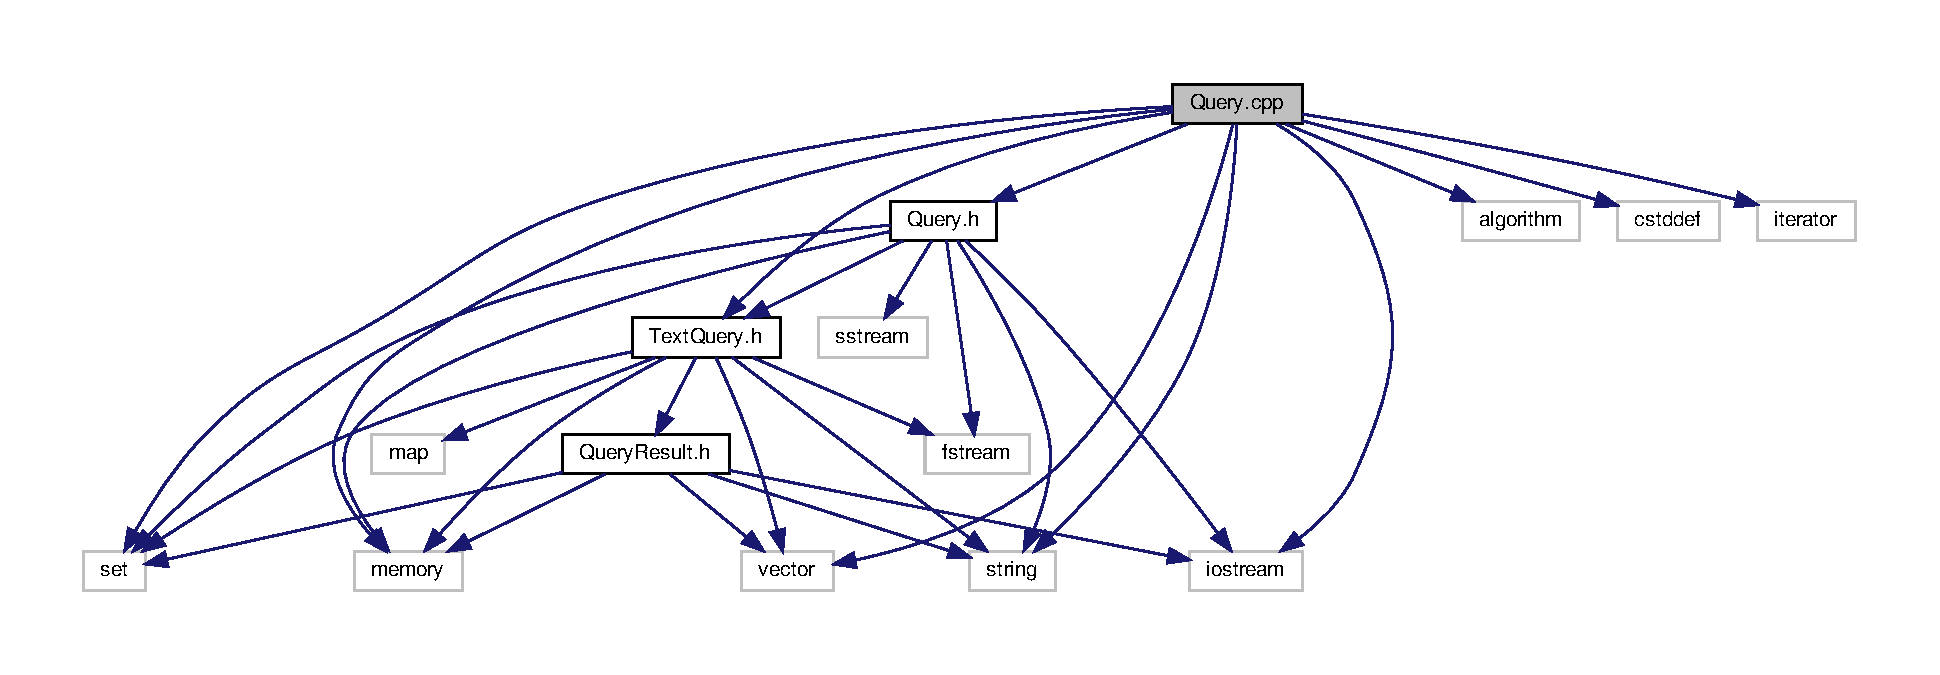
\includegraphics[width=350pt]{Query_8cpp__incl}
\end{center}
\end{figure}

\hypertarget{Query_8h}{}\section{Query.\+h 文件参考}
\label{Query_8h}\index{Query.\+h@{Query.\+h}}
{\ttfamily \#include \char`\"{}Text\+Query.\+h\char`\"{}}\newline
{\ttfamily \#include $<$string$>$}\newline
{\ttfamily \#include $<$set$>$}\newline
{\ttfamily \#include $<$iostream$>$}\newline
{\ttfamily \#include $<$fstream$>$}\newline
{\ttfamily \#include $<$sstream$>$}\newline
{\ttfamily \#include $<$memory$>$}\newline
Query.\+h 的引用(Include)关系图\+:\nopagebreak
\begin{figure}[H]
\begin{center}
\leavevmode
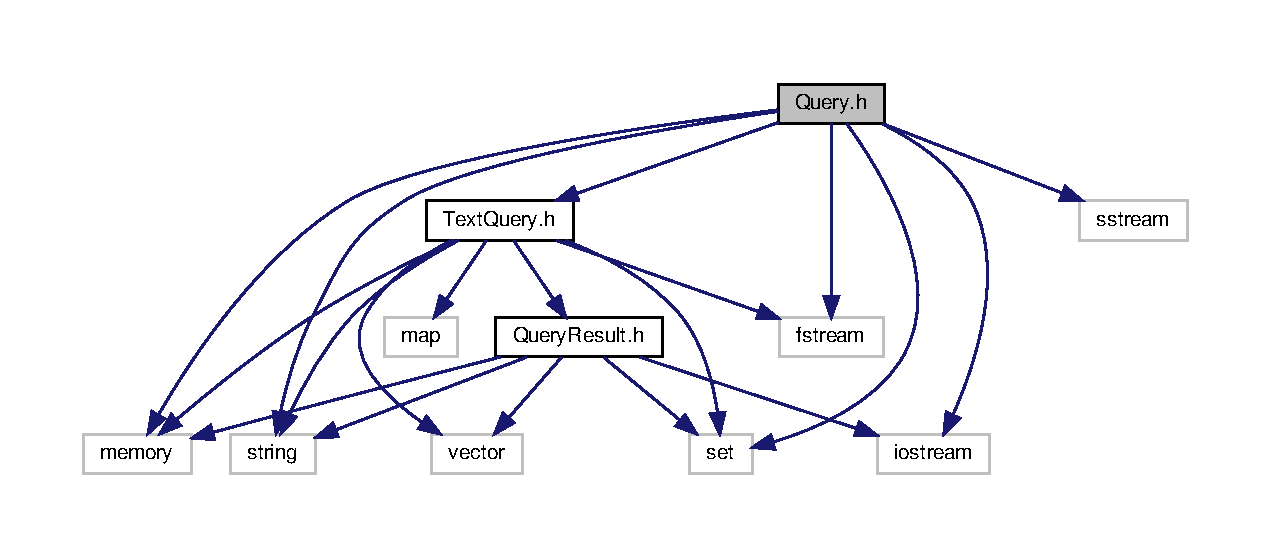
\includegraphics[width=350pt]{Query_8h__incl}
\end{center}
\end{figure}
此图展示该文件直接或间接的被哪些文件引用了\+:\nopagebreak
\begin{figure}[H]
\begin{center}
\leavevmode
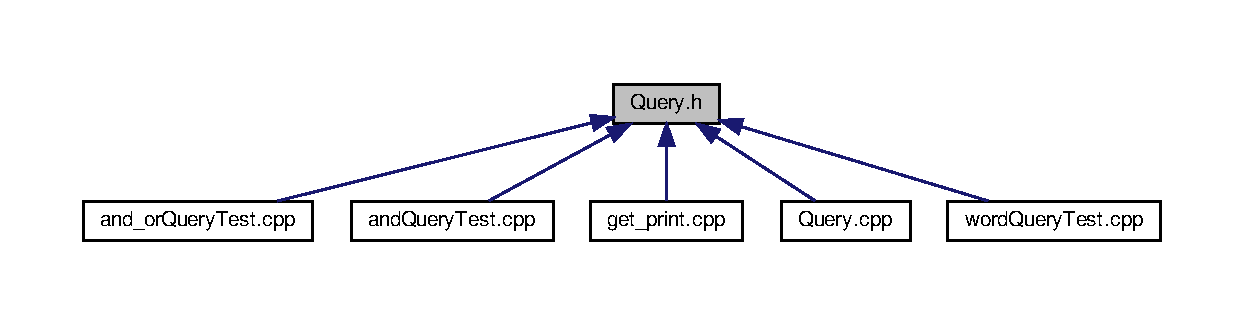
\includegraphics[width=350pt]{Query_8h__dep__incl}
\end{center}
\end{figure}
\subsection*{类}
\begin{DoxyCompactItemize}
\item 
class \hyperlink{classQuery__base}{Query\+\_\+base}
\item 
class \hyperlink{classQuery}{Query}
\item 
class \hyperlink{classWordQuery}{Word\+Query}
\item 
class \hyperlink{classNotQuery}{Not\+Query}
\item 
class \hyperlink{classBinaryQuery}{Binary\+Query}
\item 
class \hyperlink{classAndQuery}{And\+Query}
\item 
class \hyperlink{classOrQuery}{Or\+Query}
\end{DoxyCompactItemize}
\subsection*{函数}
\begin{DoxyCompactItemize}
\item 
std\+::ostream \& \hyperlink{Query_8h_abfed567a44e8bd5e953f28dfee8017b8}{operator$<$$<$} (std\+::ostream \&os, const \hyperlink{classQuery}{Query} \&query)
\item 
\hyperlink{classQuery}{Query} \hyperlink{Query_8h_ae5ac39eb549ba887f8a2fdf0b8de4bd3}{operator \&} (const \hyperlink{classQuery}{Query} \&lhs, const \hyperlink{classQuery}{Query} \&rhs)
\item 
\hyperlink{classQuery}{Query} \hyperlink{Query_8h_aa1edc8d85f1e9ad8206f20c4ff6353c2}{operator$\vert$} (const \hyperlink{classQuery}{Query} \&lhs, const \hyperlink{classQuery}{Query} \&rhs)
\item 
\hyperlink{classQuery}{Query} \hyperlink{Query_8h_a3323af056195c7641b3a80e096e5cdc3}{operator$\sim$} (const \hyperlink{classQuery}{Query} \&operand)
\item 
std\+::ifstream \& \hyperlink{Query_8h_adf8e160d906c1fcc26b5978283cb50de}{open\+\_\+file} (std\+::ifstream \&, const std\+::string \&)
\item 
\hyperlink{classTextQuery}{Text\+Query} \hyperlink{Query_8h_a3a4c9044f063867f8c5c3496e6f24270}{get\+\_\+file} (int, char $\ast$$\ast$)
\item 
bool \hyperlink{Query_8h_a3ec33b27a103bb83851fe0bae378074b}{get\+\_\+word} (std\+::string \&)
\item 
bool \hyperlink{Query_8h_ab43263517fe8aa8d750785c40fcaa9b0}{get\+\_\+words} (std\+::string \&, std\+::string \&)
\item 
std\+::ostream \& \hyperlink{Query_8h_ab20f9885050aa16c68eaeff6f8d9db7d}{print} (std\+::ostream \&, const \hyperlink{classQueryResult}{Query\+Result} \&)
\end{DoxyCompactItemize}


\subsection{函数说明}
\mbox{\Hypertarget{Query_8h_a3a4c9044f063867f8c5c3496e6f24270}\label{Query_8h_a3a4c9044f063867f8c5c3496e6f24270}} 
\index{Query.\+h@{Query.\+h}!get\+\_\+file@{get\+\_\+file}}
\index{get\+\_\+file@{get\+\_\+file}!Query.\+h@{Query.\+h}}
\subsubsection{\texorpdfstring{get\+\_\+file()}{get\_file()}}
{\footnotesize\ttfamily \hyperlink{classTextQuery}{Text\+Query} get\+\_\+file (\begin{DoxyParamCaption}\item[{int}]{,  }\item[{char $\ast$$\ast$}]{ }\end{DoxyParamCaption})}

\mbox{\Hypertarget{Query_8h_a3ec33b27a103bb83851fe0bae378074b}\label{Query_8h_a3ec33b27a103bb83851fe0bae378074b}} 
\index{Query.\+h@{Query.\+h}!get\+\_\+word@{get\+\_\+word}}
\index{get\+\_\+word@{get\+\_\+word}!Query.\+h@{Query.\+h}}
\subsubsection{\texorpdfstring{get\+\_\+word()}{get\_word()}}
{\footnotesize\ttfamily bool get\+\_\+word (\begin{DoxyParamCaption}\item[{std\+::string \&}]{ }\end{DoxyParamCaption})}

\mbox{\Hypertarget{Query_8h_ab43263517fe8aa8d750785c40fcaa9b0}\label{Query_8h_ab43263517fe8aa8d750785c40fcaa9b0}} 
\index{Query.\+h@{Query.\+h}!get\+\_\+words@{get\+\_\+words}}
\index{get\+\_\+words@{get\+\_\+words}!Query.\+h@{Query.\+h}}
\subsubsection{\texorpdfstring{get\+\_\+words()}{get\_words()}}
{\footnotesize\ttfamily bool get\+\_\+words (\begin{DoxyParamCaption}\item[{std\+::string \&}]{,  }\item[{std\+::string \&}]{ }\end{DoxyParamCaption})}

\mbox{\Hypertarget{Query_8h_adf8e160d906c1fcc26b5978283cb50de}\label{Query_8h_adf8e160d906c1fcc26b5978283cb50de}} 
\index{Query.\+h@{Query.\+h}!open\+\_\+file@{open\+\_\+file}}
\index{open\+\_\+file@{open\+\_\+file}!Query.\+h@{Query.\+h}}
\subsubsection{\texorpdfstring{open\+\_\+file()}{open\_file()}}
{\footnotesize\ttfamily std\+::ifstream\& open\+\_\+file (\begin{DoxyParamCaption}\item[{std\+::ifstream \&}]{,  }\item[{const std\+::string \&}]{ }\end{DoxyParamCaption})}

\mbox{\Hypertarget{Query_8h_ae5ac39eb549ba887f8a2fdf0b8de4bd3}\label{Query_8h_ae5ac39eb549ba887f8a2fdf0b8de4bd3}} 
\index{Query.\+h@{Query.\+h}!operator \&@{operator \&}}
\index{operator \&@{operator \&}!Query.\+h@{Query.\+h}}
\subsubsection{\texorpdfstring{operator \&()}{operator \&()}}
{\footnotesize\ttfamily \hyperlink{classQuery}{Query} operator\& (\begin{DoxyParamCaption}\item[{const \hyperlink{classQuery}{Query} \&}]{lhs,  }\item[{const \hyperlink{classQuery}{Query} \&}]{rhs }\end{DoxyParamCaption})\hspace{0.3cm}{\ttfamily [inline]}}

\mbox{\Hypertarget{Query_8h_abfed567a44e8bd5e953f28dfee8017b8}\label{Query_8h_abfed567a44e8bd5e953f28dfee8017b8}} 
\index{Query.\+h@{Query.\+h}!operator$<$$<$@{operator$<$$<$}}
\index{operator$<$$<$@{operator$<$$<$}!Query.\+h@{Query.\+h}}
\subsubsection{\texorpdfstring{operator$<$$<$()}{operator<<()}}
{\footnotesize\ttfamily std\+::ostream\& operator$<$$<$ (\begin{DoxyParamCaption}\item[{std\+::ostream \&}]{os,  }\item[{const \hyperlink{classQuery}{Query} \&}]{query }\end{DoxyParamCaption})\hspace{0.3cm}{\ttfamily [inline]}}

\mbox{\Hypertarget{Query_8h_aa1edc8d85f1e9ad8206f20c4ff6353c2}\label{Query_8h_aa1edc8d85f1e9ad8206f20c4ff6353c2}} 
\index{Query.\+h@{Query.\+h}!operator\texttt{"|}@{operator\texttt{"|}}}
\index{operator\texttt{"|}@{operator\texttt{"|}}!Query.\+h@{Query.\+h}}
\subsubsection{\texorpdfstring{operator\texttt{"|}()}{operator|()}}
{\footnotesize\ttfamily \hyperlink{classQuery}{Query} operator$\vert$ (\begin{DoxyParamCaption}\item[{const \hyperlink{classQuery}{Query} \&}]{lhs,  }\item[{const \hyperlink{classQuery}{Query} \&}]{rhs }\end{DoxyParamCaption})\hspace{0.3cm}{\ttfamily [inline]}}

\mbox{\Hypertarget{Query_8h_a3323af056195c7641b3a80e096e5cdc3}\label{Query_8h_a3323af056195c7641b3a80e096e5cdc3}} 
\index{Query.\+h@{Query.\+h}!operator$\sim$@{operator$\sim$}}
\index{operator$\sim$@{operator$\sim$}!Query.\+h@{Query.\+h}}
\subsubsection{\texorpdfstring{operator$\sim$()}{operator~()}}
{\footnotesize\ttfamily \hyperlink{classQuery}{Query} operator$\sim$ (\begin{DoxyParamCaption}\item[{const \hyperlink{classQuery}{Query} \&}]{operand }\end{DoxyParamCaption})\hspace{0.3cm}{\ttfamily [inline]}}

\mbox{\Hypertarget{Query_8h_ab20f9885050aa16c68eaeff6f8d9db7d}\label{Query_8h_ab20f9885050aa16c68eaeff6f8d9db7d}} 
\index{Query.\+h@{Query.\+h}!print@{print}}
\index{print@{print}!Query.\+h@{Query.\+h}}
\subsubsection{\texorpdfstring{print()}{print()}}
{\footnotesize\ttfamily std\+::ostream\& print (\begin{DoxyParamCaption}\item[{std\+::ostream \&}]{,  }\item[{const \hyperlink{classQueryResult}{Query\+Result} \&}]{ }\end{DoxyParamCaption})}


\hypertarget{QueryResult_8h}{}\section{Query\+Result.\+h 文件参考}
\label{QueryResult_8h}\index{Query\+Result.\+h@{Query\+Result.\+h}}
{\ttfamily \#include $<$memory$>$}\newline
{\ttfamily \#include $<$string$>$}\newline
{\ttfamily \#include $<$vector$>$}\newline
{\ttfamily \#include $<$set$>$}\newline
{\ttfamily \#include $<$iostream$>$}\newline
Query\+Result.\+h 的引用(Include)关系图\+:\nopagebreak
\begin{figure}[H]
\begin{center}
\leavevmode
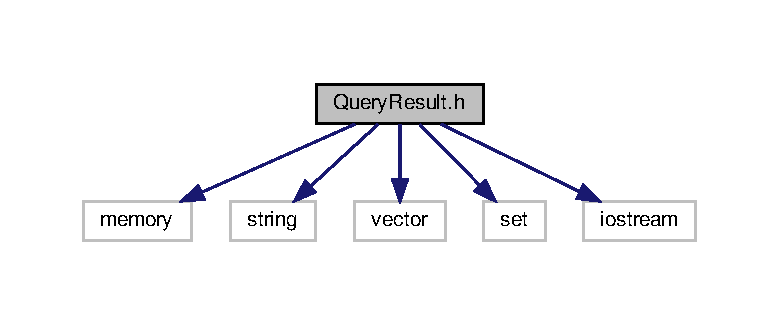
\includegraphics[width=350pt]{QueryResult_8h__incl}
\end{center}
\end{figure}
此图展示该文件直接或间接的被哪些文件引用了\+:\nopagebreak
\begin{figure}[H]
\begin{center}
\leavevmode
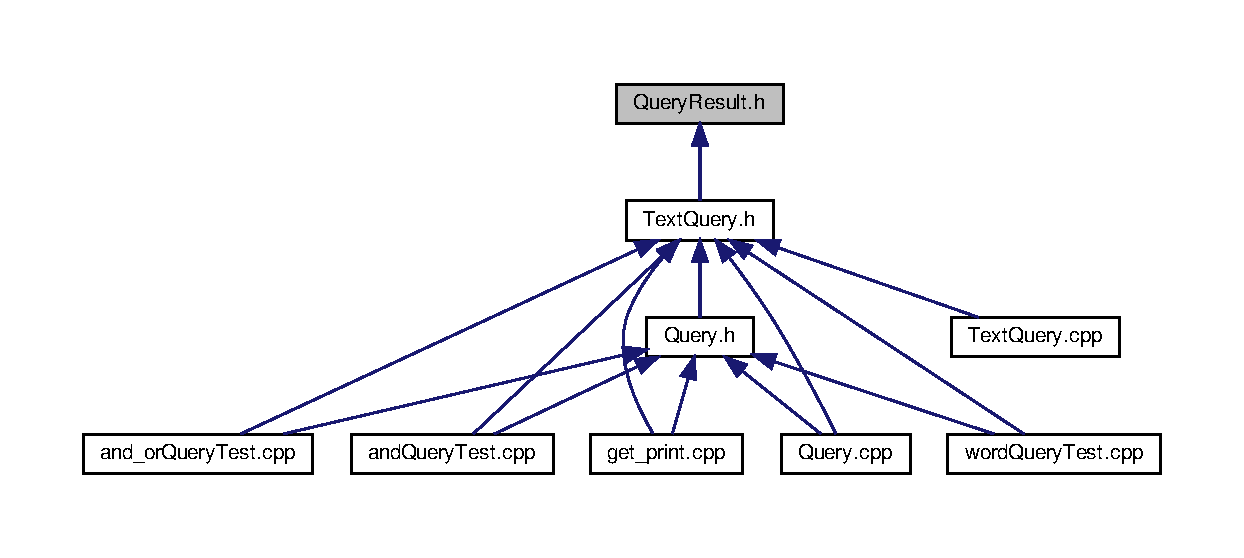
\includegraphics[width=350pt]{QueryResult_8h__dep__incl}
\end{center}
\end{figure}
\subsection*{类}
\begin{DoxyCompactItemize}
\item 
class \hyperlink{classQueryResult}{Query\+Result}
\end{DoxyCompactItemize}
\subsection*{函数}
\begin{DoxyCompactItemize}
\item 
std\+::ostream \& \hyperlink{QueryResult_8h_ab20f9885050aa16c68eaeff6f8d9db7d}{print} (std\+::ostream \&, const \hyperlink{classQueryResult}{Query\+Result} \&)
\end{DoxyCompactItemize}


\subsection{函数说明}
\mbox{\Hypertarget{QueryResult_8h_ab20f9885050aa16c68eaeff6f8d9db7d}\label{QueryResult_8h_ab20f9885050aa16c68eaeff6f8d9db7d}} 
\index{Query\+Result.\+h@{Query\+Result.\+h}!print@{print}}
\index{print@{print}!Query\+Result.\+h@{Query\+Result.\+h}}
\subsubsection{\texorpdfstring{print()}{print()}}
{\footnotesize\ttfamily std\+::ostream\& print (\begin{DoxyParamCaption}\item[{std\+::ostream \&}]{,  }\item[{const \hyperlink{classQueryResult}{Query\+Result} \&}]{ }\end{DoxyParamCaption})}


\hypertarget{TextQuery_8cpp}{}\section{Text\+Query.\+cpp 文件参考}
\label{TextQuery_8cpp}\index{Text\+Query.\+cpp@{Text\+Query.\+cpp}}
{\ttfamily \#include \char`\"{}Text\+Query.\+h\char`\"{}}\newline
{\ttfamily \#include \char`\"{}make\+\_\+plural.\+h\char`\"{}}\newline
{\ttfamily \#include $<$cstddef$>$}\newline
{\ttfamily \#include $<$memory$>$}\newline
{\ttfamily \#include $<$sstream$>$}\newline
{\ttfamily \#include $<$string$>$}\newline
{\ttfamily \#include $<$vector$>$}\newline
{\ttfamily \#include $<$map$>$}\newline
{\ttfamily \#include $<$set$>$}\newline
{\ttfamily \#include $<$iostream$>$}\newline
{\ttfamily \#include $<$fstream$>$}\newline
{\ttfamily \#include $<$cctype$>$}\newline
{\ttfamily \#include $<$cstring$>$}\newline
{\ttfamily \#include $<$utility$>$}\newline
Text\+Query.\+cpp 的引用(Include)关系图\+:\nopagebreak
\begin{figure}[H]
\begin{center}
\leavevmode
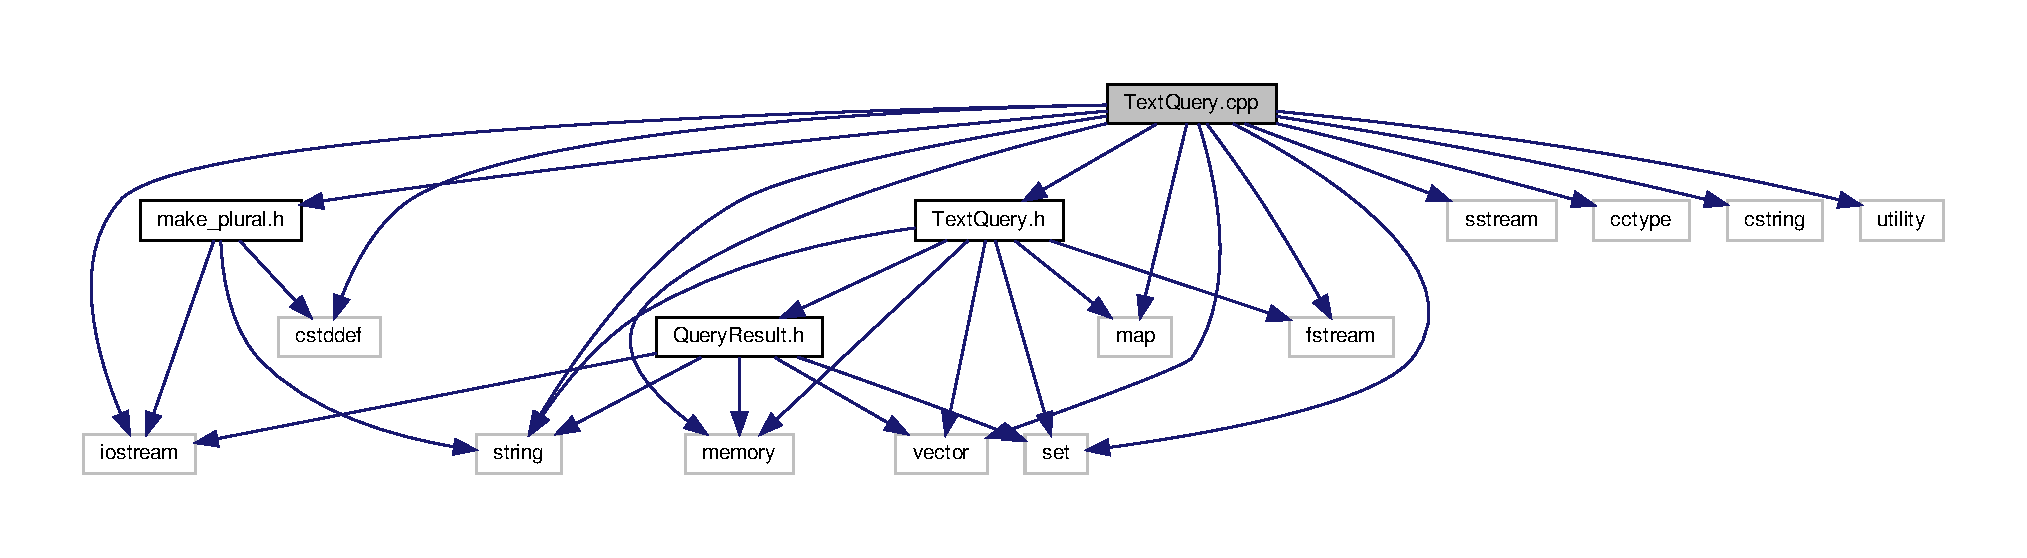
\includegraphics[width=350pt]{TextQuery_8cpp__incl}
\end{center}
\end{figure}
\subsection*{类型定义}
\begin{DoxyCompactItemize}
\item 
typedef map$<$ string, shared\+\_\+ptr$<$ set$<$ \hyperlink{classTextQuery_a504c1be8d67d4fcf4c205999e2377262}{Text\+Query\+::line\+\_\+no} $>$ $>$ $>$ \hyperlink{TextQuery_8cpp_acebdc99ff3dd51e1da2b373e7381e8b3}{wm\+Type}
\item 
typedef wm\+Type\+::const\+\_\+iterator \hyperlink{TextQuery_8cpp_ac6679374211c0e463443405e911f06ae}{wm\+Iter}
\item 
typedef shared\+\_\+ptr$<$ set$<$ \hyperlink{classTextQuery_a504c1be8d67d4fcf4c205999e2377262}{Text\+Query\+::line\+\_\+no} $>$ $>$ \hyperlink{TextQuery_8cpp_aa4e0a1113e16947c9991f221fd01eb22}{line\+Type}
\item 
typedef set$<$ \hyperlink{classTextQuery_a504c1be8d67d4fcf4c205999e2377262}{Text\+Query\+::line\+\_\+no} $>$\+::const\+\_\+iterator \hyperlink{TextQuery_8cpp_a7d0013742d5b21e5dceb51abb75b7553}{line\+Iter}
\end{DoxyCompactItemize}
\subsection*{函数}
\begin{DoxyCompactItemize}
\item 
ostream \& \hyperlink{TextQuery_8cpp_aee25760ed696efe10f8643654d9b9016}{print} (ostream \&os, const \hyperlink{classQueryResult}{Query\+Result} \&qr)
\end{DoxyCompactItemize}


\subsection{类型定义说明}
\mbox{\Hypertarget{TextQuery_8cpp_a7d0013742d5b21e5dceb51abb75b7553}\label{TextQuery_8cpp_a7d0013742d5b21e5dceb51abb75b7553}} 
\index{Text\+Query.\+cpp@{Text\+Query.\+cpp}!line\+Iter@{line\+Iter}}
\index{line\+Iter@{line\+Iter}!Text\+Query.\+cpp@{Text\+Query.\+cpp}}
\subsubsection{\texorpdfstring{line\+Iter}{lineIter}}
{\footnotesize\ttfamily typedef set$<$\hyperlink{classTextQuery_a504c1be8d67d4fcf4c205999e2377262}{Text\+Query\+::line\+\_\+no}$>$\+::const\+\_\+iterator \hyperlink{TextQuery_8cpp_a7d0013742d5b21e5dceb51abb75b7553}{line\+Iter}}

\mbox{\Hypertarget{TextQuery_8cpp_aa4e0a1113e16947c9991f221fd01eb22}\label{TextQuery_8cpp_aa4e0a1113e16947c9991f221fd01eb22}} 
\index{Text\+Query.\+cpp@{Text\+Query.\+cpp}!line\+Type@{line\+Type}}
\index{line\+Type@{line\+Type}!Text\+Query.\+cpp@{Text\+Query.\+cpp}}
\subsubsection{\texorpdfstring{line\+Type}{lineType}}
{\footnotesize\ttfamily typedef shared\+\_\+ptr$<$set$<$\hyperlink{classTextQuery_a504c1be8d67d4fcf4c205999e2377262}{Text\+Query\+::line\+\_\+no}$>$ $>$ \hyperlink{TextQuery_8cpp_aa4e0a1113e16947c9991f221fd01eb22}{line\+Type}}

\mbox{\Hypertarget{TextQuery_8cpp_ac6679374211c0e463443405e911f06ae}\label{TextQuery_8cpp_ac6679374211c0e463443405e911f06ae}} 
\index{Text\+Query.\+cpp@{Text\+Query.\+cpp}!wm\+Iter@{wm\+Iter}}
\index{wm\+Iter@{wm\+Iter}!Text\+Query.\+cpp@{Text\+Query.\+cpp}}
\subsubsection{\texorpdfstring{wm\+Iter}{wmIter}}
{\footnotesize\ttfamily typedef wm\+Type\+::const\+\_\+iterator \hyperlink{TextQuery_8cpp_ac6679374211c0e463443405e911f06ae}{wm\+Iter}}

\mbox{\Hypertarget{TextQuery_8cpp_acebdc99ff3dd51e1da2b373e7381e8b3}\label{TextQuery_8cpp_acebdc99ff3dd51e1da2b373e7381e8b3}} 
\index{Text\+Query.\+cpp@{Text\+Query.\+cpp}!wm\+Type@{wm\+Type}}
\index{wm\+Type@{wm\+Type}!Text\+Query.\+cpp@{Text\+Query.\+cpp}}
\subsubsection{\texorpdfstring{wm\+Type}{wmType}}
{\footnotesize\ttfamily typedef map$<$string, shared\+\_\+ptr$<$set$<$\hyperlink{classTextQuery_a504c1be8d67d4fcf4c205999e2377262}{Text\+Query\+::line\+\_\+no}$>$ $>$ $>$ \hyperlink{TextQuery_8cpp_acebdc99ff3dd51e1da2b373e7381e8b3}{wm\+Type}}



\subsection{函数说明}
\mbox{\Hypertarget{TextQuery_8cpp_aee25760ed696efe10f8643654d9b9016}\label{TextQuery_8cpp_aee25760ed696efe10f8643654d9b9016}} 
\index{Text\+Query.\+cpp@{Text\+Query.\+cpp}!print@{print}}
\index{print@{print}!Text\+Query.\+cpp@{Text\+Query.\+cpp}}
\subsubsection{\texorpdfstring{print()}{print()}}
{\footnotesize\ttfamily ostream\& print (\begin{DoxyParamCaption}\item[{ostream \&}]{os,  }\item[{const \hyperlink{classQueryResult}{Query\+Result} \&}]{qr }\end{DoxyParamCaption})}


\hypertarget{TextQuery_8h}{}\section{Text\+Query.\+h 文件参考}
\label{TextQuery_8h}\index{Text\+Query.\+h@{Text\+Query.\+h}}
{\ttfamily \#include $<$memory$>$}\newline
{\ttfamily \#include $<$string$>$}\newline
{\ttfamily \#include $<$vector$>$}\newline
{\ttfamily \#include $<$map$>$}\newline
{\ttfamily \#include $<$set$>$}\newline
{\ttfamily \#include $<$fstream$>$}\newline
{\ttfamily \#include \char`\"{}Query\+Result.\+h\char`\"{}}\newline
Text\+Query.\+h 的引用(Include)关系图\+:\nopagebreak
\begin{figure}[H]
\begin{center}
\leavevmode
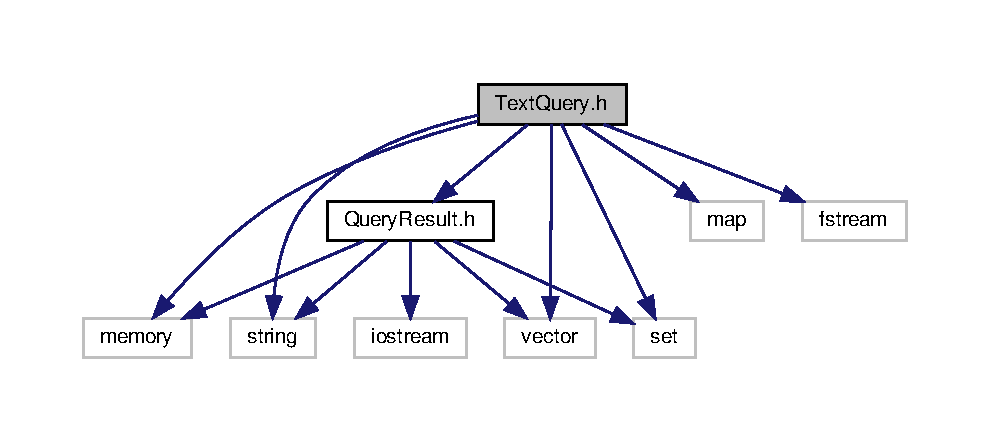
\includegraphics[width=350pt]{TextQuery_8h__incl}
\end{center}
\end{figure}
此图展示该文件直接或间接的被哪些文件引用了\+:\nopagebreak
\begin{figure}[H]
\begin{center}
\leavevmode
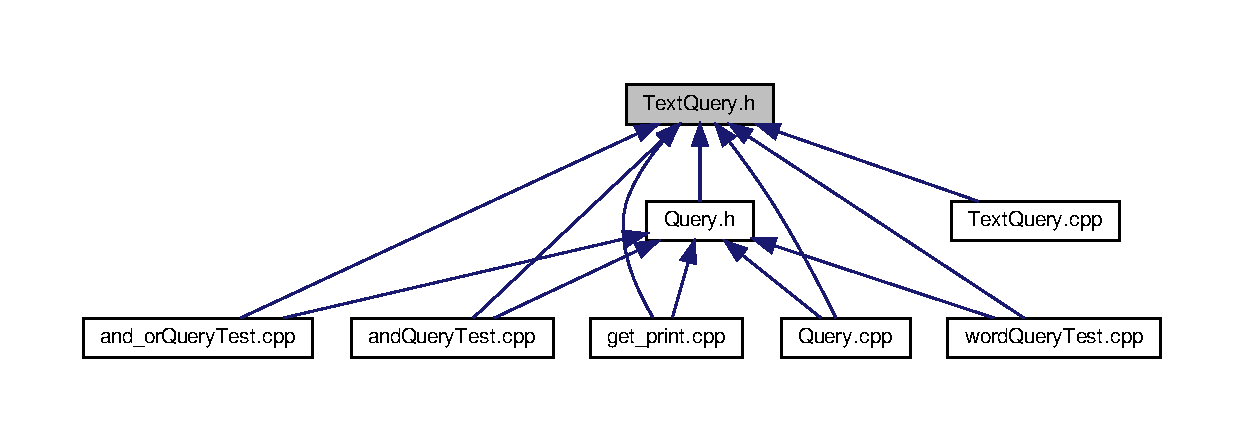
\includegraphics[width=350pt]{TextQuery_8h__dep__incl}
\end{center}
\end{figure}
\subsection*{类}
\begin{DoxyCompactItemize}
\item 
class \hyperlink{classTextQuery}{Text\+Query}
\end{DoxyCompactItemize}

\hypertarget{wordQueryTest_8cpp}{}\section{word\+Query\+Test.\+cpp 文件参考}
\label{wordQueryTest_8cpp}\index{word\+Query\+Test.\+cpp@{word\+Query\+Test.\+cpp}}
{\ttfamily \#include \char`\"{}Query.\+h\char`\"{}}\newline
{\ttfamily \#include \char`\"{}Text\+Query.\+h\char`\"{}}\newline
{\ttfamily \#include $<$string$>$}\newline
{\ttfamily \#include $<$vector$>$}\newline
{\ttfamily \#include $<$map$>$}\newline
{\ttfamily \#include $<$set$>$}\newline
{\ttfamily \#include $<$iostream$>$}\newline
{\ttfamily \#include $<$fstream$>$}\newline
{\ttfamily \#include $<$cctype$>$}\newline
{\ttfamily \#include $<$cstring$>$}\newline
word\+Query\+Test.\+cpp 的引用(Include)关系图\+:\nopagebreak
\begin{figure}[H]
\begin{center}
\leavevmode
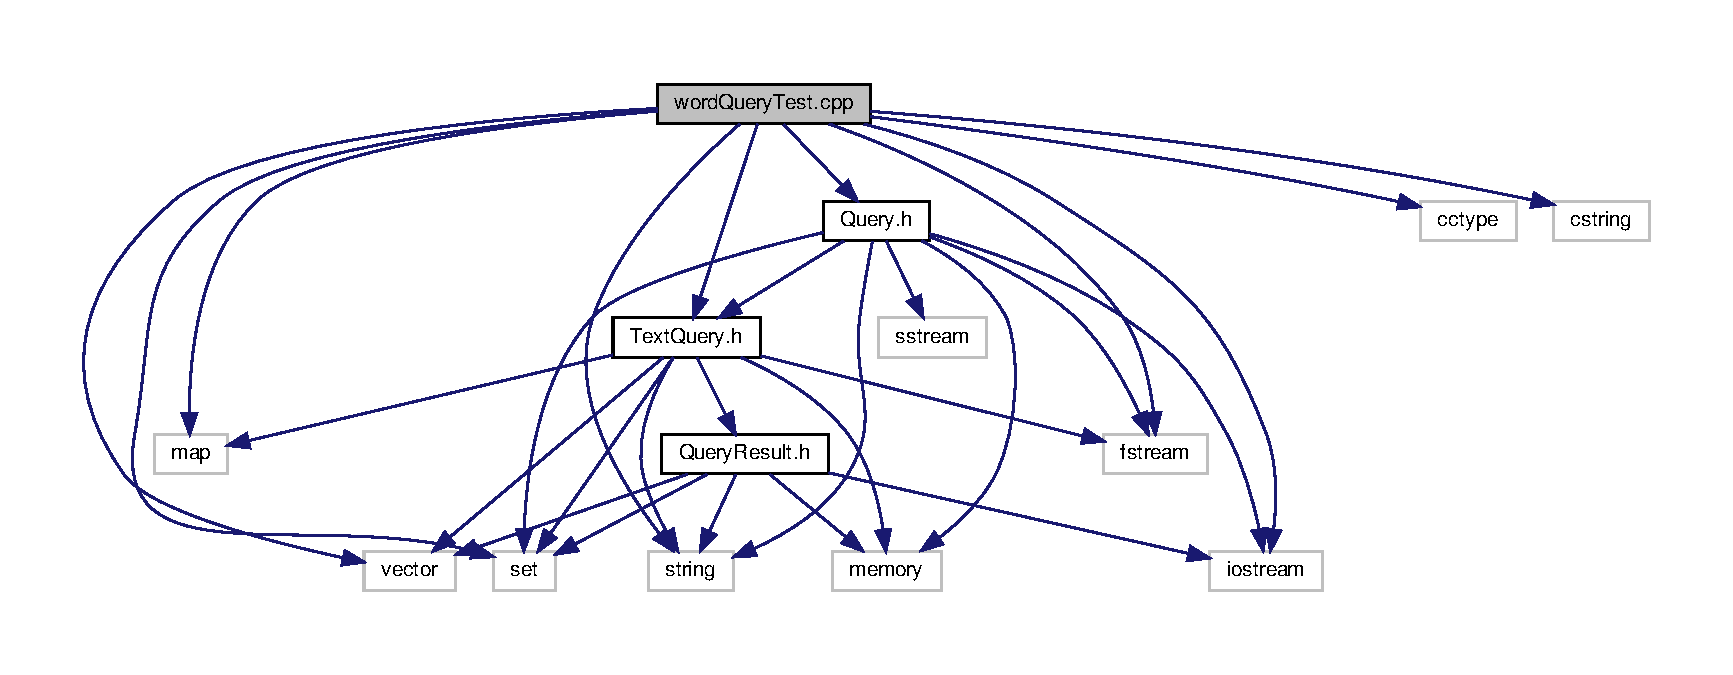
\includegraphics[width=350pt]{wordQueryTest_8cpp__incl}
\end{center}
\end{figure}
\subsection*{函数}
\begin{DoxyCompactItemize}
\item 
int \hyperlink{wordQueryTest_8cpp_a3c04138a5bfe5d72780bb7e82a18e627}{main} (int argc, char $\ast$$\ast$argv)
\end{DoxyCompactItemize}


\subsection{函数说明}
\mbox{\Hypertarget{wordQueryTest_8cpp_a3c04138a5bfe5d72780bb7e82a18e627}\label{wordQueryTest_8cpp_a3c04138a5bfe5d72780bb7e82a18e627}} 
\index{word\+Query\+Test.\+cpp@{word\+Query\+Test.\+cpp}!main@{main}}
\index{main@{main}!word\+Query\+Test.\+cpp@{word\+Query\+Test.\+cpp}}
\subsubsection{\texorpdfstring{main()}{main()}}
{\footnotesize\ttfamily int main (\begin{DoxyParamCaption}\item[{int}]{argc,  }\item[{char $\ast$$\ast$}]{argv }\end{DoxyParamCaption})}


%--- End generated contents ---

% Index
\backmatter
\newpage
\phantomsection
\clearemptydoublepage
\addcontentsline{toc}{chapter}{索引}
\printindex

\end{document}
